\documentclass[12pt]{article}
\usepackage[utf8]{inputenc}
\usepackage[T1]{fontenc}
\usepackage{amsmath}
\usepackage{amssymb}
\usepackage{amsthm}
\usepackage{geometry}
\geometry{margin=1in}
\usepackage{setspace}
\usepackage[hypertexnames=false]{hyperref}
\usepackage{booktabs}
\usepackage{graphicx}
\usepackage{float}
\usepackage{enumitem}
\setlist{itemsep=2pt, parsep=2pt}
\doublespacing

\newtheorem{proposition}{Proposition}
\newtheorem{definition}{Definition}

% Math macros
\newcommand{\kB}{k_{\mathrm{B}}}
\newcommand{\Teff}{T_{\mathrm{eff}}}
\newcommand{\Deff}{D_{\mathrm{eff}}}

\title{Coherence time in biological oscillator assemblies bounds the rate of state registration}

\author{Ian Todd\\
Sydney Medical School, University of Sydney\\
Sydney, NSW, Australia\\
\texttt{itod2305@uni.sydney.edu.au}}

\date{1 March 2026}

\begin{document}

\maketitle

\begin{abstract}
The physical principles determining how fast distributed neural assemblies can synchronize---and thus how fast the neural processes underlying cognition can proceed---remain incompletely formalized. We derive a coherence time bound for coupled oscillator networks: the minimum interval between irreversible state registrations (``commits'') scales exponentially with coordination depth $M$. For $M$ semi-independent modules requiring phase alignment at coherence $r$, the commit rate is dominated by rare-event first-passage time on the configuration torus, producing a fundamental speed-flexibility trade-off---increasing $M$ expands combinatorial flexibility but slows commits exponentially; increasing $r$ accelerates synchronization but restricts dynamics to lower-dimensional manifolds. Kuramoto simulations validate the expected scaling in modular networks ($R^2 = 0.97$) and delineate regime boundaries in all-to-all and sparse topologies. Using independently constrained parameters, the framework recovers the empirical 30--50 ms visual binding window and shows that coordination time dominates quantum, thermodynamic, and power limits in biological neural systems by many orders of magnitude. We also develop exploratory extensions of the framework: a pre-commit ``phase delta'' regime in which structured phase offsets bias downstream outcomes before registration, candidate biophysical substrates for that regime, and qualitative predictions for alpha entrainment, stress-related temporal distortion, and pharmacological modulation of subjective time. The central claim is therefore modest and testable: in systems with identifiable modular coordination architecture, multi-module phase alignment can be the dominant rate-limiting step on biological processing.
\end{abstract}

\textbf{Keywords:} biological oscillations, coherence time, coordination depth, temporal resolution, quantum speed limits, Landauer bound, coupled oscillators

\section{Introduction}

\subsection{Processing speed in biological oscillator assemblies}

A fundamental insight from systems neuroscience is that cognition emerges from coherent oscillations across neural assemblies, not merely from individual spike rates. Working memory maintenance involves theta-gamma phase-amplitude coupling organized in discrete oscillatory bursts~\cite{miller2018,lisman2013,lundqvist2016}. Attention selectively enhances inter-areal synchronization in gamma band~\cite{fries2015,womelsdorf2007}. Perceptual binding depends on transient phase alignment across visual cortices~\cite{singer1999,engel2001}. Long-range communication occurs preferentially during coherent states~\cite{varela2001}. The ``communication through coherence'' framework~\cite{fries2005} has become central to understanding neural computation.

Yet despite extensive empirical characterization, the physical principles governing \emph{how fast} distributed assemblies can achieve coherence---and thus how quickly the neural processes underlying cognitive operations can proceed---remain incompletely formalized. Why does perceptual binding require 30--50 ms rather than 3 ms or 300 ms? Why do larger assemblies integrating more information process more slowly? What determines the relationship between oscillation frequency and temporal acuity?

\subsection{Coherence time as a physical bound on processing rate}

Recent work argued that living intelligence is an emergent property of high-dimensional, self-sustaining dynamical systems that maintain coherence against decoherence~\cite{todd2025intelligence}, building on analyses of falsifiability limits in adaptive biological systems~\cite{todd2025biosystems} and timing inaccessibility in sub-Landauer computation~\cite{todd2025demon}. The present manuscript addresses the complementary question: given such a coherent high-dimensional system, what sets the fastest timescale on which it can register change and update its state?

We formalize this as the minimum interval between irreversible ``commit'' events:
transitions in which distributed dynamics become readable to downstream mechanisms,
consistent with the emerging view that perception operates in discrete cycles~\cite{vanrullen2016}.
This commit interval is bounded by a coordination term
(coherence time as a first-passage problem on a product manifold)
together with quantum, noise, and power limits.

\textbf{Operational definition of commits in neural systems.} A state registration (or ``commit'') is operationally detected when distributed oscillatory dynamics cross a threshold that enables stable downstream readout. Empirical signatures include: (i) phase-locking index exceeding threshold across specified modules for a minimum duration, (ii) onset of stable cross-frequency coupling (e.g., theta-gamma PAC), and (iii) classifier-detectable state transition in downstream neural populations. The framework addresses the temporal resolution of such events; it does not claim that all neural computation reduces to discrete registrations.

\begin{definition}[Commit event]\label{def:commit}
Given $M$ modules with aggregate phases $\psi_1(t), \ldots, \psi_M(t)$ and within-module coherences $r_{\mathrm{intra},m}(t)$, a \textbf{commit} occurs at time $t^*$ if:
\begin{enumerate}
\item All modules are internally coherent: $r_{\mathrm{intra},m}(t^*) \geq r_{\mathrm{thr}}$ for all $m$.
\item Phases are mutually aligned: $\max_m |\psi_m(t^*) - \bar{\psi}(t^*)| \leq \varepsilon/2$, where $\bar{\psi}$ is the circular mean.
\item The alignment persists for dwell time $T_{\mathrm{dwell}}$.
\end{enumerate}
The commit is defined \emph{relative to a downstream readout mechanism}; different readouts may have different $(r_{\mathrm{thr}}, \varepsilon, T_{\mathrm{dwell}})$ parameters.
\end{definition}

\textbf{Empirical proxies for commit detection:} PLI threshold crossing (sustained $r_{\mathrm{inter}} > r_{\mathrm{thresh}}$), PAC onset, or classifier-detectable state change. These are measurement definitions; different tasks may require different readout criteria.

\medskip

\noindent\fbox{\parbox{\dimexpr\linewidth-2\fboxsep-2\fboxrule}{%
\textbf{Minimal empirical pipeline.}
To estimate coherence time from neural data:
\begin{enumerate}[noitemsep]
\item Identify modules via connectivity/functional clustering $\to$ count $M$
\item Extract module-level phases $\psi_m(t)$ via Hilbert transform or band-pass filtering
\item Compute intra- and inter-module coherence: $r_{\mathrm{intra}}, r_{\mathrm{inter}}$
\item Define alignment threshold $\varepsilon$ from task requirements (e.g., decoding accuracy)
\item Estimate attempt rate $\lambda_{\mathrm{attempt}}$ from decorrelation time of $r_{\mathrm{inter}}(t)$
\item Measure first-passage times to sustained alignment $\to$ fit Eq.~\ref{eq:coh-time}
\end{enumerate}}}

\textbf{Definition (Physical dimensionality).} Throughout this work, ``dimensionality'' refers to the effective degrees of freedom of accessible dynamics---not geometric embedding dimension. Physical dimensionality is a quantitative measure of effective connectivity: how many independent directions of coordinated variation are accessible to a system given its interaction structure. High-dimensional states correspond to weakly constrained dynamics in which many components vary semi-independently; low-dimensional states correspond to strongly coupled dynamics restricted to a small number of collective modes. Dimensionality in this sense is determined not by component count, but by the rank of the system's interaction structure. Different measurement schemes (participation ratios, manifold dimension, information-geometric metrics) estimate this property from data~\cite{amari2016}.

Physical dimensionality is state-dependent: the same system may occupy high- or low-dimensional regimes depending on coupling strength and task demands. Coherence time depends on how many semi-independent constraints must be simultaneously satisfied for a commit to occur---not on any particular estimator.

\textbf{Operationalizing dimensionality.} Physical dimensionality must be estimated from measurable quantities. For the coherence time framework, we operationalize effective dimensionality as:
\begin{enumerate}
\item \textbf{Coordination depth $M$}: Count of semi-independent modules (functional clusters) whose order parameters must jointly exceed threshold. Estimated via community detection on band-limited coherence networks or anatomical parcellation.
\item \textbf{Effective independence $\alpha$}: Fraction of potential constraint dimensions that are actually independent. Estimated via:
\begin{itemize}
\item Participation ratio of module-phase covariance (Eq.~\ref{eq:deff-estimator}),
\item or empirical scaling of $\tau$ with $M$ across task conditions.
\end{itemize}
\item \textbf{Effective constraint dimension}: $d_{\mathrm{eff}} = \alpha(M-1)$ represents the number of semi-independent coordination requirements for a commit.
\end{enumerate}
These are \emph{estimators} of the underlying physical property. Future work may employ other proxies (information-geometric metrics, topological data analysis, dynamical systems dimension estimates), but the coherence time itself depends on the physical constraint structure, not the measurement method.

\subsection{Structure of this work}

We first derive the coherence time formula from principles of phase synchronization in coupled oscillator networks (\S2.1), then characterize the speed-flexibility trade-off (\S2.2). Section 2.3 introduces an exploratory interpretation of the pre-commit interval in terms of structured phase-delta dynamics. Section 2.4 situates the framework within the hierarchy of physical limits on computation, addressing the Landauer bound, Margolus-Levitin quantum speed limit, and energy-time uncertainty relation. Section 2.5 provides parameter estimation protocols. Section 3 applies the framework to neural systems, demonstrating quantitative agreement with perceptual binding windows, tachypsychia dissociations, and metabolic scaling. Section 4 discusses generalization, exploratory extensions, limitations, and testable predictions.

\section{Theory and Methods}

\subsection{The unified temporal resolution bound}

We model biological temporal processing as a sequence of \emph{commits}---thermodynamically irreversible events that register high-dimensional internal state as low-dimensional output. A commit requires: (1) dimensional collapse from distributed state ($\Deff$ dimensions) to registered outcome (few dimensions), (2) dissipation of at least $\kB T \ln 2$ per bit (Landauer bound), and (3) creation of a persistent measurement influencing future dynamics.

The minimum time between commits is bounded below by four physical constraints:

\begin{equation}\label{eq:main-bound}
\boxed{\tau_{\mathrm{eff}} \;\gtrsim\; \max\left[\tau_{\mathrm{QSL}},\; \tau_{\mathrm{SNR}},\; \tau_{\mathrm{coh}},\; \tau_{\mathrm{power}}\right]}
\end{equation}

This is a \textbf{lower bound}: the effective commit interval must be at least as long as the slowest constraint. The max operation is appropriate when these constraints act on largely independent subsystems that can be satisfied in parallel (e.g., quantum state evolution, signal detection, and phase coordination proceed concurrently). If constraints were strictly sequential (e.g., signal detection \emph{then} coordination \emph{then} dissipation), a sum would be more appropriate. In biological neural systems, the constraints are largely parallel, and the coherence time dominates by orders of magnitude, so the distinction has minimal practical impact.

\textbf{Epistemic status.} $\tau_{\mathrm{QSL}}$ and the Landauer energy-per-bit are hard physical bounds; $\tau_{\mathrm{SNR}}$ and $\tau_{\mathrm{power}}$ are model-dependent; $\tau_{\mathrm{coh}}$ is an asymptotic rare-event estimate whose scaling exponent $(M-1)$ is robust but whose prefactor requires calibration. The key claim is not that Eq.~\ref{eq:main-bound} is a theorem, but that $\tau_{\mathrm{coh}}$ dominates by orders of magnitude, making the precise form of other constraints largely irrelevant.

The four terms are:

\paragraph{Quantum speed limit ($\tau_{\mathrm{QSL}}$).} The Mandelstam-Tamm and Margolus-Levitin bounds~\cite{mandelstam1945,margolus1998} establish
\[
\tau_{\mathrm{QSL}} = \max\left[\frac{\hbar}{2\Delta E},\; \frac{\pi\hbar}{2\langle E\rangle}\right]
\]
For biological temperatures ($\Delta E \sim \kB T$), $\tau_{\mathrm{QSL}} \sim 10^{-13}$ s.

\paragraph{Signal-to-noise limit ($\tau_{\mathrm{SNR}}$).} In additive white Gaussian noise with two-sided power spectral density $N_0$ over bandwidth $B$, matched-filter detection achieves $\mathrm{SNR}(T) = 2P_s T/N_0$, where $P_s$ is signal power and $T$ is integration time~\cite{poor1994}. Reaching detection threshold $\rho_{\min} \sim 5$--10 then requires
\[
\tau_{\mathrm{SNR}} = \frac{\rho_{\min} N_0}{2P_s}
\]

\paragraph{Power limit ($\tau_{\mathrm{power}}$).} Dimensional collapse by $\Delta\mathcal{D}$ at dimensional chemical potential $\lambda_{\mathcal{D}} \sim \kB\Teff$ costs energy $\sim \lambda_{\mathcal{D}}\Delta\mathcal{D}$. At sustained power $P$, commit rate is bounded by
\[
\tau_{\mathrm{power}} = \frac{\lambda_{\mathcal{D}}\Delta\mathcal{D}}{P}
\]
For cortical visual binding: $\Delta\mathcal{D} \sim 50$ (participation ratio of visual cortex assemblies collapsing to a $\sim$5-bit readout), $\lambda_{\mathcal{D}} \geq \kB T \ln 2 \approx 3 \times 10^{-21}$~J (Landauer floor), and $P \sim 10^{-4}$~W (power budget of a $\sim$$10^4$-neuron cortical assembly at $\sim$10~nW/neuron). This yields $\tau_{\mathrm{power}} \sim 10^{-15}$~s at the Landauer minimum. Biological neurons are energetically inefficient: ion-channel computation dissipates $\sim$$10^7$ times the Landauer floor per degree of freedom~\cite{landauer1961}. Even at this biophysical scale, $\tau_{\mathrm{power}} \sim 10^{-8}$~s---still six orders of magnitude below $\tau_{\mathrm{coh}}$. The power limit is therefore non-binding in the neural regime.

\paragraph{Coherence time ($\tau_{\mathrm{coh}}$).}
We model commits as threshold crossings requiring $M$ semi-independent modules to achieve simultaneous phase alignment within tolerance $\varepsilon$, building on the theory of coupled oscillators~\cite{kuramoto1984,acebron2005}.
Let $r$ denote the \textbf{inter-module coherence} $r_{\mathrm{inter}} = |M^{-1}\sum_m e^{i\psi_m}|$ where $\psi_m$ is the aggregate phase of module $m$. (We reserve $r_{\mathrm{global}}$ for the all-oscillator order parameter, which serves as a diagnostic but does not appear in Eq.~\ref{eq:coh-time}.) The von Mises concentration $\kappa(r)$ satisfies $r=I_1(\kappa)/I_0(\kappa)$~\cite{mardia2000}.

\textbf{Why von Mises?} Given circular symmetry and a fixed mean resultant length $r$, the maximum-entropy distribution on the circle is von Mises~\cite{mardia2000}. This makes our modeling choice the canonical least-informative closure: $r \to \kappa \to p_1$ is uniquely determined without additional distributional assumptions. We validate this closure empirically in simulation (conditional-on-$r$ fitting yields $\kappa_{\mathrm{fitted}}/\kappa_{\mathrm{expected}} = 1.06 \pm 0.12$).

\textbf{Definition of alignment event.} We define alignment relative to the \textbf{instantaneous mean phase} $\bar{\psi} = \arg(\sum_m e^{i\psi_m})$: all modules must fall within $\varepsilon/2$ of $\bar{\psi}$. Formally:
\[
A_\varepsilon = \{|\psi_m - \bar{\psi}| < \varepsilon/2 \text{ for all } m\}
\]
This definition is natural for empirical detection (threshold on max phase deviation from mean) and matches our simulation event detector. Because the mean phase $\bar{\psi}$ is determined by the configuration itself, we have $M-1$ independent constraints (the mean absorbs one degree of freedom).

The alignment probability is:
\[
P(A_\varepsilon) \approx p_1(\varepsilon, \kappa)^{M-1}
\]
where $p_1(\varepsilon, \kappa) = \int_{-\varepsilon/2}^{\varepsilon/2} \frac{e^{\kappa\cos\theta}}{2\pi I_0(\kappa)} d\theta$ is the single-variable window probability under von Mises$(\kappa)$.

\textbf{Remark (alternative reference definitions).} One can also define alignment relative to an anchored reference (e.g., a pacemaker module $\theta_1$) or a random reference. These alternatives yield the same $(M-1)$ scaling exponent, differing only by $O(1)$ constants. We use the mean-phase definition throughout because it matches empirical practice and our simulation protocol.

In all cases:
\begin{equation}\label{eq:coh-mises}
P(A_\varepsilon) \propto p_1(\varepsilon, \kappa)^{M-1}
\end{equation}

\textbf{Small-$\varepsilon$ approximation.} For small windows, the von Mises density near the mode gives $p_1(\varepsilon, \kappa) \approx \varepsilon \cdot e^\kappa / (2\pi I_0(\kappa))$, yielding:
\[
\tau_{\mathrm{coh}} \approx \frac{1}{\lambda_{\mathrm{attempt}}} \left( \frac{2\pi I_0(\kappa)}{\varepsilon \, e^\kappa} \right)^{\alpha(M-1)}
\]
This makes the $\varepsilon^{-\alpha(M-1)}$ scaling and the ``exponential in $M$'' dependence explicit. Here $\lambda_{\mathrm{attempt}}$ (s$^{-1}$) is the effective alignment attempt rate, estimated from the decorrelation time of inter-module phase coherence $r_{\mathrm{inter}}(t)$ (see below). \emph{Note:} We use the exact $p_1(\varepsilon, \kappa)$ integral for all numerical estimates (e.g., the binding window calculations use $\varepsilon = \pi/2$); the small-$\varepsilon$ expansion is presented only to clarify the scaling structure.

\textbf{The exponent is $(M-1)$, not $M$.} This arises from quotient geometry: the reference module $\theta_1$ serves as anchor (whether fixed or conditioned upon), leaving $M-1$ independent constraints. This is analogous to the classic result that the probability of $M$ uniform phases falling in \emph{some} semicircle is $M/2^{M-1}$, where the factor $M$ accounts for the free choice of arc location; our anchored definition removes this degree of freedom.

\textbf{Generalization to arbitrary phase constraints.} The alignment event need not be ``all phases near a common reference.'' More generally, suppose a commit requires $k$ independent phase constraints to be satisfied, where each constraint has marginal probability $p_i$ (e.g., specific phase lags between area pairs, cluster relationships, or cross-frequency conditions). Then:
\[
P(\text{alignment}) = \prod_{i=1}^k p_i \approx \bar{p}^k
\]
where $\bar{p}$ is the geometric mean probability. The coherence time scales as $\tau_{\mathrm{coh}} \propto \bar{p}^{-k}$, i.e., exponentially in the number of constraints. Our ``all within $\varepsilon/2$ of mean'' definition is a special case with $k = M-1$ and $p_i = p_1(\varepsilon, \kappa)$. The framework applies whenever commits require multiple semi-independent conditions to be simultaneously satisfied.

\textbf{First-passage time structure.} Assuming independence across modules on the commit timescale, the alignment event $A_\varepsilon$ is a rare target set on the $M$-torus $T^M$. Under fast mixing relative to the target set size, first-passage times are approximately exponential with mean $\tau \approx 1/(\text{attempt rate} \times P(A_\varepsilon))$---a form of Kac's recurrence theorem~\cite{kac1947}.

\begin{proposition}[First-passage time under mixing]\label{prop:fpt}
Let $X(t)$ be an ergodic Markov process on state space $\mathcal{X}$ with stationary distribution $\pi$ and mixing time $\tau_{\mathrm{mix}}$ (the time for $\|P_t(x, \cdot) - \pi\|_{\mathrm{TV}} \leq 1/4$ from worst-case initial state). For a target set $A \subset \mathcal{X}$ with $\pi(A) \ll 1$, the hitting time $T_A = \inf\{t : X(t) \in A\}$ satisfies:
\[
\mathbb{E}[T_A] \approx \frac{\tau_{\mathrm{mix}}}{\pi(A)} \quad \text{as } \pi(A) \to 0.
\]
Moreover, $T_A / \mathbb{E}[T_A]$ is approximately exponentially distributed when $\pi(A) \ll 1$.
\end{proposition}
\noindent This is a standard result in the theory of rare events for Markov chains~\cite{kac1947,levinperes2017}. The key assumptions are ergodicity and that the process mixes on timescales much shorter than the expected hitting time. In our setting, ``mixing'' means that successive phase configurations separated by $\tau_{\mathrm{mix}}$ are approximately independent samples from the stationary distribution; hence the Bernoulli-trial heuristic: each mixing interval is an independent ``attempt'' to land in $A_\varepsilon$.

\textbf{Attempt rate.} Let $\tau_{\mathrm{mix}}$ denote the mixing time of the joint phase process---the timescale on which phase configurations become approximately independent of their initial state. The effective number of independent ``alignment attempts'' per unit time is $\sim 1/\tau_{\mathrm{mix}}$. We define the \textbf{attempt rate}:
\[
\lambda_{\mathrm{attempt}} \equiv \frac{1}{\tau_{\mathrm{mix}}} \quad \text{(units: s}^{-1}\text{)}
\]
This is \emph{not} the carrier frequency of oscillations, but the rate at which the relative-phase configuration effectively ``resamples.''

We estimate $\lambda_{\mathrm{attempt}}$ from the inverse decorrelation time of the inter-module order parameter $z_{\mathrm{inter}}(t) = \frac{1}{M}\sum_m e^{i\psi_m(t)}$, where $\psi_m(t)$ is the mean phase of module $m$. The decorrelation time $\tau_{\mathrm{mix}}$ is defined as the $1/e$ crossing of the autocorrelation function of $|z_{\mathrm{inter}}(t)|$, and $\lambda_{\mathrm{attempt}} = 1/\tau_{\mathrm{mix}}$.

\textbf{Units convention.} We report $\lambda_{\mathrm{attempt}}$ in s$^{-1}$. When using the spectral spread proxy, $\Delta\omega$ (rad/s) is the standard deviation of instantaneous phase velocities; the corresponding frequency spread is $\Delta f = \Delta\omega/(2\pi)$ in Hz. In weakly-coupled regimes, $\lambda_{\mathrm{attempt}} \approx \Delta\omega$ (since the radian is dimensionless, $\Delta\omega$ in rad/s and $\lambda_{\mathrm{attempt}}$ in s$^{-1}$ are directly comparable); equivalently, $\lambda_{\mathrm{attempt}} \approx 2\pi\Delta f$.

\textbf{Simulation proxy.} In simulations, $\lambda_{\mathrm{attempt}}$ is measured directly from the autocorrelation of $|z_{\mathrm{inter}}(t)|$, which gives $1/\tau_{\mathrm{mix}}$ in s$^{-1}$ without angular ambiguity. The spectral spread proxy is used only as a consistency check. For neural data analysis, we recommend estimating $\lambda_{\mathrm{attempt}}$ from the autocorrelation time of inter-module phase deviations, which directly measures the mixing timescale.

This yields:
\begin{equation}\label{eq:coh-time-exact}
\tau_{\mathrm{coh}} = \frac{1}{\lambda_{\mathrm{attempt}}}\,p_1(\varepsilon, \kappa(r))^{-(M-1)}
\end{equation}

Relaxing the independence assumption in Eq.~\ref{eq:coh-time-exact} for coupled modules, the effective exponent is reduced:
\begin{equation}\label{eq:coh-time}
\boxed{\tau_{\mathrm{coh}} \approx \frac{1}{\lambda_{\mathrm{attempt}}}\,p_1(\varepsilon, \kappa(r))^{-\alpha(M-1)}},\qquad \alpha\in(0,1],
\end{equation}
where $\alpha$ captures \emph{effective independence} (a correlation-reduction exponent: $\alpha = 1$ for fully independent modules, $\alpha < 1$ when inter-module coupling induces correlations that reduce the effective number of constraints).

\textbf{Estimating effective constraint dimension.} Define the \textbf{effective constraint dimension}:
\[
d_{\mathrm{eff}} = \alpha(M-1)
\]
This can be estimated from the covariance structure of module phases. Let $C$ be the $M \times M$ covariance matrix of phase deviations $\delta\psi_m = \psi_m - \bar{\psi}$. The \textbf{participation ratio} provides an operational estimate:
\begin{equation}\label{eq:deff-estimator}
\hat{d}_{\mathrm{eff}} = \frac{(\mathrm{tr}\, C)^2}{\mathrm{tr}(C^2)} = \frac{\left(\sum_i \lambda_i\right)^2}{\sum_i \lambda_i^2}
\end{equation}
where $\lambda_i$ are eigenvalues of $C$. Participation-ratio and related manifold-based summaries are standard empirical tools for quantifying effective neural dimensionality~\cite{cunningham2014,stringer2019}. Because $\delta\psi_m$ are mean-centred ($\sum_m \delta\psi_m = 0$), $C$ has rank at most $M-1$; the participation ratio therefore equals $M-1$ when all non-zero eigenvalues are equal (fully independent) and approaches 1 when a single mode dominates (fully correlated). From $\hat{d}_{\mathrm{eff}}$, we obtain $\hat{\alpha} = \hat{d}_{\mathrm{eff}} / (M-1)$.

\textbf{Why correlations affect the exponent.}
For independent phase deviations $\delta\psi_m$ with uniform distribution over $[-\pi, \pi]$,
the probability of all $M$ modules aligning within $\pm\varepsilon/2$ scales as $\sim \varepsilon^{M-1}$.
However, when deviations are correlated with effective rank $d_{\mathrm{eff}}$,
the measure of a small alignment neighborhood scales like $\varepsilon^{d_{\mathrm{eff}}}$
(up to constants depending on the correlation structure).
Hence the exponent is effectively $d_{\mathrm{eff}}$, motivating $\alpha(M-1) \approx d_{\mathrm{eff}}$.
This is analogous to the effective dimensionality of a correlated Gaussian:
if $\mathbf{X} \sim \mathcal{N}(0, \Sigma)$ with eigenvalues $\lambda_i$,
the volume of an $\varepsilon$-ball scales like $\varepsilon^{d_{\mathrm{eff}}}$ where
$d_{\mathrm{eff}} = (\sum_i \lambda_i)^2 / \sum_i \lambda_i^2$ (participation ratio).

\textbf{Relationship between PR and scaling exponent.} The participation ratio estimates the effective rank of the phase covariance matrix, while $\alpha$ in Eq.~\ref{eq:coh-time} modifies an exponent in a rare-event probability on the torus. These are related but not identical: the PR gives the effective rank of correlations, while the scaling exponent depends on how that rank translates into target-set measure. The PR provides an upper bound on the effective constraint dimension, with approximate equality when the eigenvalue structure maps linearly onto alignment probability---which holds for moderate coherence ($r \sim 0.3$--$0.7$) but may break down at extremes (very low $r$, where all eigenvalues are nearly equal, or very high $r$, where conditioning on the dominant mode becomes important). The supplementary validation (Test 3) shows empirical agreement within 15\% across the moderate-coherence regime, supporting the use of PR as an operational estimator of $\alpha(M-1)$.

\textbf{Log-linear form.} Taking logarithms makes the exponential-in-$M$ scaling explicit:
\[
\log \tau_{\mathrm{coh}} = -\log \lambda_{\mathrm{attempt}} - \alpha(M-1)\log p_1(\varepsilon, \kappa(r)).
\]
Since $p_1 < 1$, we have $-\log p_1 > 0$, so coherence time grows exponentially with effective constraint dimension $\alpha(M-1)$.

\begin{figure}[H]
\centering
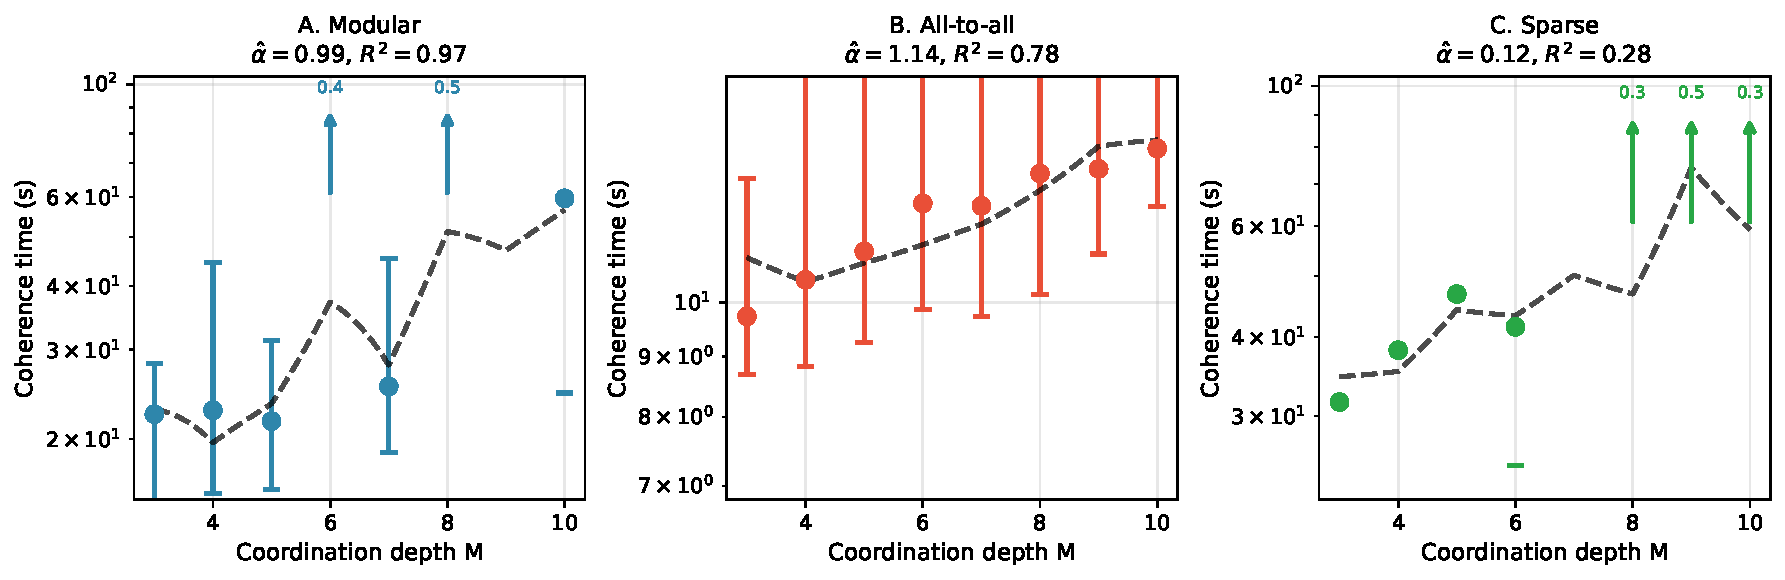
\includegraphics[width=\textwidth]{simulations/figures/fig1.pdf}
\caption{\textbf{Coherence time scaling: validation (modular) and regime-boundary diagnostics (all-to-all, sparse).}
(A) Modular, (B) All-to-all, (C) Sparse random networks ($N=100$ oscillators, $K=0.7$, $\varepsilon=1.0$ rad, 20 trials per $M$).
Points show median coherence time $\tau_{\mathrm{coh}}$ with interquartile ranges (error bars).
For heavily censored points whose Kaplan-Meier median exceeds the 60 s observation window, upward arrows indicate lower bounds beginning at that observation horizon; fully censored $M$ values (no commits observed) are omitted.
We fit Eq.~\ref{eq:coh-time} using two approaches: (i)~\textbf{theory-consistent}:
$\log(\tau \cdot \lambda_{\mathrm{attempt}}) = \alpha(M-1)[-\log p_1(\varepsilon, \kappa(\bar{r}_{\mathrm{inter}}))] + c$
using the trajectory-mean inter-module coherence $\bar{r}_{\mathrm{inter}}$ (averaged over all trials, including censored, to estimate the stationary distribution), and
(ii)~\textbf{linearized surrogate}:
$\log(\tau \cdot \lambda_{\mathrm{attempt}}) \approx \alpha \cdot \tilde{c} \cdot (1-\bar{r}_{\mathrm{inter}})(M-1) + c'$
for comparison.
Dashed lines show fitted predictions with $\hat{\alpha}$ and $R^2$ values indicated.
The three topologies serve as validation (modular) and regime-boundary diagnostics (all-to-all, sparse).
\textbf{Modular networks} ($\hat{\alpha} \approx 1$, $R^2 = 0.97$, $n=5$ $M$-values): near-independent modules, the regime where the theory's assumptions are best satisfied and validation is strongest.
\textbf{All-to-all coupling} ($\hat{\alpha} \approx 1$ via linearized surrogate, $n=8$): regime-boundary diagnostic; theory-consistent fit is ill-conditioned where $\bar{r}_{\mathrm{inter}} \approx 1$ makes $-\log p_1 \approx 0$.
\textbf{Sparse random networks} ($\hat{\alpha} \approx 0.1$, $R^2 = 0.28$, $n=4$): regime-boundary diagnostic; strong correlations collapse effective constraints, confirming that modular architecture is a necessary condition for the scaling law, not an incidental feature of the validation.}
\label{fig:topology}
\end{figure}

\textbf{Key assumptions.} Equation~\ref{eq:coh-time} relies on:
\begin{enumerate}
\item \textbf{Stationarity}: The phase distribution is approximately stationary over the commit timescale.
\item \textbf{Fast mixing}: The joint phase process mixes rapidly relative to the target set size, so first-passage times are approximately exponential (memoryless after conditioning on slowly varying parameters like $r$).
\item \textbf{Weak coupling}: Modules are semi-independent on the commit timescale; strong coupling would synchronize phases and reduce effective $M$.
\item \textbf{Attempt rate interpretation}: $\lambda_{\mathrm{attempt}}$ represents the inverse correlation time of phase deviations, not the carrier frequency.
\end{enumerate}
\textbf{Diagnostic}: If these assumptions hold, inter-commit intervals (after conditioning on $r$) should be approximately exponentially distributed. Deviations indicate strong coupling, metastability, or non-stationarity. Supplementary simulations support this diagnostic (Fig.~\ref{fig:conditional-exponentiality}): waiting times conditioned on narrow $r_{\mathrm{inter}}$ bins are approximately exponential (Kolmogorov-Smirnov test), though the analysis conditions on observed hits rather than the full censored survival process.

\textbf{Dwell time and the scaling analysis.} Definition~\ref{def:commit} requires alignment to persist for a dwell time $T_{\mathrm{dwell}}$. This introduces a ``hold probability'' $q(T_{\mathrm{dwell}}; r)$---the probability that alignment, once achieved, survives for duration $T_{\mathrm{dwell}}$. The effective commit rate becomes $\lambda_{\mathrm{attempt}} \cdot P(A_\varepsilon) \cdot q$, so $q$ renormalizes the prefactor but does not alter the exponential-in-$M$ scaling, which is driven entirely by $P(A_\varepsilon)$. In simulations we enforce dwell explicitly; for the scaling analysis, $q$ is absorbed into $\lambda_{\mathrm{attempt}}$ as a constant-factor correction and estimated empirically from decorrelation of $|z_{\mathrm{inter}}(t)|$.

\textbf{Simulation limitation.} In the modular Kuramoto validation (Fig.~\ref{fig:topology}), we vary $M$ at fixed total population $N$, which changes module size ($\sim N/M$). This can introduce finite-size effects and alter within- vs between-module coupling balance. For cleaner $M$-scaling, one would keep module size constant by scaling $N$ with $M$. Despite this limitation, the exponential scaling with $M$ is strong in modular networks ($R^2=0.97$) and qualitatively consistent in all-to-all and sparse topologies, though quantitative fit quality degrades where the theory's modularity assumptions are violated (see caption, Fig.~\ref{fig:topology}).

\textbf{Heavy-tailed waiting times.} Empirically observed inter-commit intervals may exhibit heavy tails even when the underlying process is well-described by Eq.~\ref{eq:coh-time}. This arises naturally when $r(t)$, $\lambda_{\mathrm{attempt}}(t)$, or network state drift slowly relative to the commit timescale. The marginal waiting time distribution then becomes a \emph{mixture of exponentials} (a Cox or doubly stochastic process), which can produce power-law-like tails. The key testable prediction is that waiting times \emph{conditional on a narrow bin of $r$} should remain approximately exponential, even when the unconditional distribution is heavy-tailed.

\begin{figure}[H]
\centering
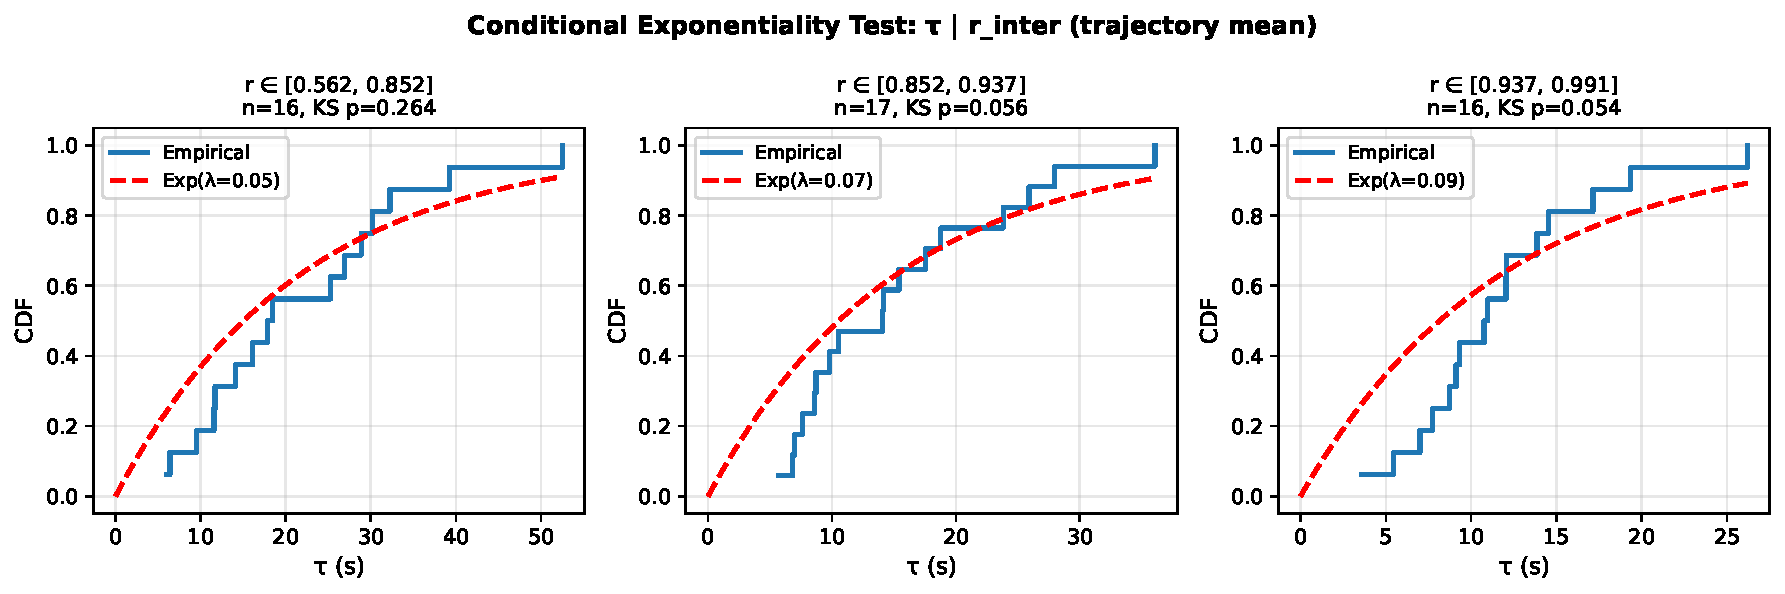
\includegraphics[width=0.85\textwidth]{simulations/figures/fig2.pdf}
\caption{\textbf{Conditional exponentiality diagnostic.}
Unconditional inter-commit interval distributions can appear heavy-tailed. Conditioning on narrow bins of inter-module coherence $r_{\mathrm{inter}}$ among observed commits yields approximately exponential waiting times within each bin (Kolmogorov-Smirnov test), consistent with a mixture-of-exponentials interpretation in which slow drift of $r(t)$ broadens the marginal waiting-time distribution. Because this analysis conditions on observed hits, it should be read as a diagnostic rather than a full survival-model validation.}
\label{fig:conditional-exponentiality}
\end{figure}

\textbf{Interpretation.} $M$ is the coordination depth:
the number of semi-independent modules (functional clusters) whose order parameters
must jointly exceed a threshold for a commit to register. \emph{Modules are not individual oscillators}:
within-module coherence is absorbed into the module's aggregate phase estimate.
$\lambda_{\mathrm{attempt}}$ is the attempt rate: the characteristic rate at which
inter-module phases decorrelate and ``resample'' rather than the carrier frequency.
The tolerance $\varepsilon$ is the full phase window width (in radians);
$\varepsilon = \pi/2$ corresponds to $\pm 45^\circ$ alignment tolerance,
typical for gamma-band binding.

\textbf{Foundational assumption: continuous coordination variables.} This framework focuses on continuous phase variables as the coordination substrate. The commit definition, alignment probabilities, and rare-event statistics are naturally expressed in phase coordinates because phases can \emph{explore} configuration space between commits---the core requirement for the first-passage geometry we model.

If commits are discrete state registrations (spike cascades, readout events) and the phase delta regime is interpreted as continuous, high-dimensional exploration between commits, then one should look for a comparably continuous coordination substrate. This constrains the candidate substrates. Chemical synaptic transmission requires presynaptic spikes and involves quantal vesicle release; neuromodulators are comparatively slow for oscillatory coordination; and gap junctions, while continuous, are sparse in cortex. A plausible candidate is therefore the \textbf{extracellular electric field}: it is continuous in space and time, spatially extended across modules, and measurable via local field potentials. Ephaptic coupling~\cite{anastassiou2011,pinotsis2023,han2018} provides one mechanism by which such field structure could modulate spike timing.

This should be read as a working biophysical hypothesis, not as a theorem forced by the mathematics. The coherence-time framework requires some continuous coordination variable, but it does not by itself prove that extracellular fields are the unique substrate. Synaptic, dendritic, and other subthreshold state variables may also participate. The narrower claim is that field-level measurements are a natural place to look for pre-commit phase structure if such structure is functionally significant.

Field effects are causally plausible because extracellular electric fields modulate membrane potential, and membrane potential influences spike timing~\cite{anastassiou2011}. The open empirical question is therefore not whether field effects exist, but how much they matter relative to synaptic coupling in a given regime~\cite{anastassiou2011,beggs2003,shew2013}. The framework suggests a specific dependency: the functional impact of small timing perturbations should grow with effective dimensionality $\Deff$, because higher-dimensional phase structure creates more semi-independent timing relationships through which weak perturbations can propagate.

\subsection{The speed-flexibility trade-off}

The coherence time reveals opposing constraints on commit rate:

\begin{proposition}[Speed-Flexibility Frontier]\label{prop:tradeoff}
At fixed power $P$, systems face a Pareto frontier in $(M,r)$ space:
\begin{itemize}
\item \textbf{Increasing $M$}: Expands combinatorial flexibility (number of modules whose phases can vary independently) but slows commits via $\tau_{\mathrm{coh}} \propto (\mathrm{const})^{M}$
\item \textbf{Increasing $r$}: Speeds commits via reduced circular variance $(1-r)$ but restricts exploration to low-dimensional synchronized manifold
\end{itemize}
\end{proposition}

Increasing coordination depth $M$ expands the dimensionality of commit-registered outcomes but requires exponentially longer alignment time. Increasing $r_{\mathrm{inter}}$ reduces the dimensionality of the \textbf{relative-phase degrees of freedom}, constraining dynamics toward a lower-dimensional \textbf{phase-synchronized manifold}~\cite{strogatz2000,ott2008}. This makes multi-module coordination faster (larger $p_1$) but reduces the number of effectively independent constraints (smaller effective $\alpha$).

Importantly, this does not imply that \textbf{all} neural activity becomes low-dimensional; amplitude patterns, cross-frequency interactions, and within-module heterogeneity can remain rich. The dimensionality reduction refers specifically to the inter-module phase coordination subspace.

\subsection{The phase delta regime: computation before commitment}

The coherence time formula (Eq.~\ref{eq:coh-time}) describes the waiting time for simultaneous multi-module alignment. A natural reading treats the pre-commit interval as passive exploration---random phase diffusion until alignment occurs by chance. A more interesting possibility is that some of this interval is computationally structured rather than merely idle.

\begin{definition}[Phase delta regime]\label{def:phase-delta}
The \textbf{phase delta regime} is the dynamical state in which inter-module phase differences $\Delta\psi_{mn}(t) = \psi_m(t) - \psi_n(t)$ are maintained in structured (non-uniform) configurations that persist over timescales longer than $1/\lambda_{\mathrm{attempt}}$ but do not satisfy the alignment criterion $|\Delta\psi_{mn}| < \varepsilon$ for all pairs. Formally, the system occupies the phase delta regime when:
\begin{enumerate}
\item Phase differences are \emph{structured}: the distribution of $\{\Delta\psi_{mn}\}$ is non-uniform, concentrated near preferred offsets that reflect coupling topology and recent history.
\item Phase differences are \emph{not locked}: inter-module coherence $r_{\mathrm{inter}}$ remains bounded away from 1, preserving degrees of freedom in the relative-phase subspace.
\item The configuration \emph{biases future commits}: the conditional probability of commit outcomes given current phase differences differs from the unconditional probability.
\end{enumerate}
\end{definition}

In this regime, the system can be interpreted as performing \emph{analog computation}: evolving phase relationships between modules continuously update which commit outcomes are accessible, without yet registering a discrete state. On that interpretation, the commit is not the computation itself but the \emph{readout} of computation that has already occurred in the phase-delta interval.

A system with $M$ modules spends most of its time outside committed states. The fraction of time spent in committed states scales as $P(A_\varepsilon) \propto p_1^{\alpha(M-1)}$, which for biologically relevant parameters ($M \sim 8$, $p_1 \sim 0.7$, $\alpha \sim 0.7$) gives $P(A_\varepsilon) \sim 0.15$. The remaining $\sim 85\%$ of dynamics therefore occurs in the broader pre-commit regime. If the phase-delta interpretation is correct, much of the biasing dynamics occurs there rather than at the commit itself.

\paragraph{Bias without collision.} The standard neural oscillation literature treats phase synchrony as a \emph{binding} mechanism: when phases lock, information from different modules is bound into a unified representation~\cite{singer1999,fries2005}. The phase delta framework suggests a different interpretation. The computationally relevant regime is not phase locking itself but the \emph{approach to} phase locking---the interval during which structured phase relationships bias downstream dynamics without collapsing to a committed state.

This distinction matters because bias and binding have different computational signatures:
\begin{itemize}
\item \textbf{Binding} (phase locking, $r_{\mathrm{inter}} \to 1$): Collapses inter-module phase degrees of freedom. The system occupies a low-dimensional synchronized manifold. Downstream readout is possible, but combinatorial flexibility is lost.
\item \textbf{Biasing} (structured phase deltas, intermediate $r_{\mathrm{inter}}$): Maintains inter-module phase degrees of freedom while constraining their distribution. The system explores a high-dimensional configuration space with \emph{anisotropic} probability---some commit outcomes become more accessible than others without being determined.
\end{itemize}

\noindent\textbf{Biophysical mechanism of pre-commit bias.} How might structured phase relationships influence downstream circuits before a commit occurs? One plausible route is through extracellular-field modulation of excitability: oscillatory phase can bias membrane potential via ephaptic effects~\cite{anastassiou2011,fries2005}, so structured inter-module phase offsets may create spatially patterned gain fields in downstream targets even without synchronous firing. Such bias could then be consolidated through more conventional synaptic mechanisms, including subthreshold dendritic integration and short-term synaptic facilitation or depression. On this reading, the field-mediated component is graded and reversible, while synaptic consolidation provides the persistence needed for eventual commit.

The speed-flexibility trade-off (Proposition~\ref{prop:tradeoff}) can now be restated in terms of the phase delta regime: increasing $r$ accelerates the transition \emph{from} the phase delta regime \emph{to} a commit, but shortens the duration of analog computation available before commitment. Systems that commit too quickly lose the computational benefit of exploring the phase delta regime; systems that never commit fail to register outcomes for downstream use.

\paragraph{Sub-Landauer operation of the phase delta regime.} If the phase-delta interval is genuinely analog and pre-committal, then its maintenance need not incur the per-bit Landauer cost associated with irreversible erasure. Landauer's principle~\cite{landauer1961} applies to logically irreversible operations---specifically, erasure or overwriting of a discrete state. By contrast, maintaining a structured phase relationship can be interpreted as continuous biasing of future outcomes prior to readout. The relevant energy cost is then the coupling energy required to sustain that bias, not necessarily a per-bit erasure cost.

This interpretation is consistent with the analysis of timing inaccessibility in continuous biological substrates~\cite{todd2025demon}: systems with continuous state variables can bias future trajectories without crossing a discrete erasure threshold, because intermediate states need not be destroyed. Within that framing, the coherence time $\tau_{\mathrm{coh}}$ quantifies how long such bias can be maintained before the accumulated phase relationships either commit (alignment within $\varepsilon$) or decorrelate (bias dissipates).

\paragraph{Discrete structure from continuous dynamics.} A natural objection is that intelligence produces discrete structure---phoneme boundaries, categorical percepts, motor primitives, genetic codes---and that this discreteness implies fundamentally combinatorial computation. The phase delta framework resolves this tension: discrete structure is not the substrate of computation but its \emph{output}, emerging at commits where $M-1$ continuous phase degrees of freedom collapse to a low-dimensional registered state. Code formation---the appearance of a finite alphabet of distinguishable outputs---is an emergent property of dimensional collapse, not an architectural prerequisite (see Theorem~2 in~\cite{todd2025intelligence}). Combinatorial explosion is a property of \emph{low-dimensional, collision-dense} systems; high-dimensional continuous dynamics avoid it because trajectories generically do not collide~\cite{todd2025intelligence}. The phase delta regime exploits this collision-free geometry to bias outcomes without combinatorial branching; discrete structure and combinatorial power appear only at the commit interface.

\subsection{Quantum and thermodynamic limits of computation}

How does the coordination-based framework relate to fundamental physical limits? Three bounds are relevant. Landauer's principle~\cite{landauer1961,bormashenko2024} requires dissipation of at least $\kB T \ln 2 \approx 3 \times 10^{-21}$ J per irreversible bit at biological temperature---an energy constraint, not a time constraint. The Margolus-Levitin theorem~\cite{margolus1998} and Mandelstam-Tamm relation~\cite{mandelstam1945} together establish the quantum speed limit $\tau_{\mathrm{QSL}} = \max[\pi\hbar/(2\langle E\rangle),\; \hbar/(2\Delta E)]$, originating from the energy-time uncertainty relation $\Delta E \cdot \Delta t \gtrsim \hbar/2$~\cite{khrennikov2021,igamberdiev2025constraints,igamberdiev2026autopoietic}. As Bormashenko~\cite{bormashenko2024} notes, synthesis of these bounds yields a minimal computation time $\tau_{\min} \sim h/\kB T$. At biological temperatures ($\langle E\rangle \sim \kB T$), $\tau_{\mathrm{QSL}} \sim 10^{-13}$ s.

The hierarchy for cortical visual processing is:
\begin{align}
\tau_{\mathrm{QSL}} &\sim 10^{-13} \text{ s} \quad \text{(quantum speed limit)} \\
\tau_{\mathrm{power}} &\sim 10^{-15}\text{--}10^{-8} \text{ s} \quad \text{(power limit; see \S2.1)} \\
\tau_{\mathrm{SNR}} &\sim 10^{-3} \text{ s} \quad \text{(signal detection)} \\
\tau_{\mathrm{coh}} &\sim 10^{-2} \text{ s} \quad \text{(coordination time)}
\end{align}

For neural-scale energies, QSL and Landauer bounds are far below observed cognitive timescales; they are not rate-limiting in this regime. The gap (approximately eleven orders of magnitude) arises because neural computation is not limited by how fast individual elements switch states, but by how long distributed assemblies take to achieve coordinated phase alignment. Even modest coordination ($M \sim 5$--15) produces millisecond-scale coherence times from microsecond-scale phase dynamics. Quantum and thermodynamic bounds set absolute floors that any physical process must respect, but biological neural systems operate in a regime where multi-module coordination provides the binding constraint on processing rate.

\subsection{Parameter estimation protocols}

\paragraph{Coordination depth ($M$).} $M$ is the count of semi-independent modules whose order parameters must jointly exceed a threshold to register a commit.
\textbf{Operational estimation:}
\begin{enumerate}
\item Cluster channels/units by band-limited coherence or Granger causality into modules.
\item Identify the minimal set of modules whose joint activity predicts behavioral commits.
\item Typical values: occipital visual tasks yield $M \sim 6$--10; cross-modal binding $M \sim 10$--15.
\end{enumerate}

\paragraph{Coherence parameter ($r$).} Extract instantaneous phase $\theta_j(t)$ from bandpass-filtered LFP/EEG via Hilbert transform. For the coherence time model, we distinguish:
\begin{itemize}
\item \textbf{Within-module coherence:} $r_{\mathrm{intra},m}(t) = \left|\frac{1}{n_m}\sum_{j \in m} e^{i\theta_j(t)}\right|$ for module $m$ with $n_m$ channels.
\item \textbf{Inter-module coherence:} $r_{\mathrm{inter}}(t) = \left|\frac{1}{M}\sum_{m=1}^M e^{i\psi_m(t)}\right|$ where $\psi_m$ is module $m$'s aggregate phase.
\end{itemize}
Commits require high $r_{\mathrm{intra}}$ (modules are internally coherent) \emph{and} rare alignment of inter-module phases (low baseline $r_{\mathrm{inter}}$, with commits occurring when $r_{\mathrm{inter}}$ transiently exceeds threshold). The $r$ and $\kappa$ in Eq.~\ref{eq:coh-time} refer to the \emph{inter-module} distribution. Typical inter-module values: spontaneous cortex $\sim 0.2$--0.4; attention $\sim 0.5$--0.7~\cite{fries2015,womelsdorf2007}.

\textbf{Interpretation of $r$ in Eq.~\ref{eq:coh-time}.} The parameter $r$ can be interpreted in two ways: (1) as a slowly varying \emph{state variable} $r(t)$, in which case Eq.~\ref{eq:coh-time} gives an instantaneous hazard rate $h(t) = \lambda_{\mathrm{attempt}}\, p_1^{\alpha(M-1)}$, and the waiting time distribution becomes a hazard integral over the trajectory of $r(t)$; or (2) as a \emph{conditional} parameter representing coherence during the pre-commit interval, in which case Eq.~\ref{eq:coh-time} gives the mean waiting time conditional on that coherence level. Interpretation (1) naturally explains heavy-tailed waiting time distributions when $r(t)$ drifts slowly.

\paragraph{Phase alignment window ($\varepsilon$).} From spike train or LFP cross-correlograms, measure half-width at half-maximum (HWHM, units: seconds). The \textbf{full} phase window is $\varepsilon = 2\,\omega_0\,\mathrm{HWHM}$ (radians).

\paragraph{Attempt rate ($\lambda_{\mathrm{attempt}}$).} Estimate from the decorrelation time of inter-module coherence $|z_{\mathrm{inter}}(t)|$: $\lambda_{\mathrm{attempt}} = 1/\tau_{\mathrm{mix}}$ (s$^{-1}$). Alternatively, estimate from instantaneous frequency spread: $\lambda_{\mathrm{attempt}} \approx \Delta\omega$ (rad/s $\equiv$ s$^{-1}$, since rad is dimensionless), equivalently $\lambda_{\mathrm{attempt}} \approx 2\pi\Delta f$ where $\Delta f$ is in Hz. Typical values for cortical alpha/beta bands: $\lambda_{\mathrm{attempt}} \sim 60$--$200$ s$^{-1}$, corresponding to frequency spreads $\Delta f \sim 10$--$30$ Hz (i.e., $\Delta\omega \sim 60$--$190$ rad/s).

\textbf{Practical limitation.} The $1/e$ crossing of an autocorrelation function is notoriously noisy for short time series. In simulations we use long stationary trajectories ($T = 60$ s, $\sim 10^4$ samples); for real EEG recordings of comparable length, non-stationarity of $r(t)$ will degrade the estimate. A windowed approach---computing $\lambda_{\mathrm{attempt}}$ in sliding epochs and reporting the distribution---would be more robust for empirical application. The frequency-spread proxy ($\lambda_{\mathrm{attempt}} \approx \Delta\omega$) provides a less precise but more stable alternative for short recordings.

\textbf{Analysis workflow summary.} To apply the coherence time framework to neural data:
\begin{enumerate}
\item \textbf{Define modules}: Use community detection on coherence matrices, or anatomical ROIs.
\item \textbf{Compute module phases}: Extract $\psi_m(t)$ from bandpass-filtered signals via Hilbert transform; verify within-module coherence $r_{\mathrm{intra},m} \geq r_{\mathrm{thr}}$.
\item \textbf{Compute inter-module coherence}: $r_{\mathrm{inter}}(t) = |M^{-1}\sum_m e^{i\psi_m(t)}|$; convert to $\kappa$ via $r = I_1(\kappa)/I_0(\kappa)$.
\item \textbf{Estimate $\varepsilon$}: Measure cross-correlogram HWHM; $\varepsilon = 2\omega_0 \cdot \mathrm{HWHM}$.
\item \textbf{Estimate $\lambda_{\mathrm{attempt}}$}: Compute autocorrelation of $|z_{\mathrm{inter}}(t)|$; set $\lambda_{\mathrm{attempt}} = 1/\tau_{\mathrm{mix}}$ where $\tau_{\mathrm{mix}}$ is the $1/e$ crossing. \textbf{Recommended practice:} use a windowed approach (sliding epochs) and report the distribution of $\lambda_{\mathrm{attempt}}$ estimates, to handle non-stationarity in real recordings.
\item \textbf{Avoid outcome leakage}: When estimating $r_{\mathrm{inter}}$ for use in Eq.~\ref{eq:coh-time}, use the trajectory-mean coherence (averaged over the full recording, including non-commit intervals), not $r$ measured at or near commit time. The latter is selection-biased upward (high precisely because alignment occurred) and inflates $p_1$ estimates.
\item \textbf{Fit $\alpha$}: Either from participation ratio of module-phase covariance (Eq.~\ref{eq:deff-estimator}), or from scaling of $\tau$ with $M$ across task conditions.
\end{enumerate}

\section{Results}

\subsection{Visual perceptual binding windows}

\textbf{Censoring note.} For simulation trials that did not reach the alignment threshold within simulation time $T$, we treat these as right-censored observations and report Kaplan-Meier survival estimates of $\tau_{\mathrm{coh}}$. Points with hit fraction $< 0.5$ and at least one observed commit are shown as lower bounds with upward arrows beginning at $T$; fully censored $M$ values are omitted.

Human visual perception exhibits temporal integration windows of 30--50 ms for perceptual binding tasks. Note that critical flicker fusion (CFF) thresholds are higher ($\sim$60 Hz photopic) for simple luminance detection---a low-$M$ task requiring minimal inter-module coordination. The gap between CFF and binding-window timescales is itself predicted by the framework: low-$M$ commits are fast; high-$M$ perceptual binding is slow. We apply Eq.~\ref{eq:main-bound} with neural parameters for the high-$M$ binding case.

\textbf{Parameter provenance:} We take $M=8$ occipital modules (a plausible count of functional submodules in visual binding, including V1, V2, V4, and posterior parietal subdivisions; can be estimated via community detection on coherence networks). Coherence $r=0.7$--$0.8$ reflects attentional engagement~\cite{fries2015}. Full tolerance $\varepsilon=\pi/2$ rad ($\pm 45^\circ$) corresponds to the phase windows observed in gamma-band cross-correlograms during visual binding; note that $\pm 90^\circ$ tolerance would be too loose for functional synchrony. Attempt rate $\lambda_{\mathrm{attempt}} \approx 60$--$200$ s$^{-1}$ is estimated from the decorrelation time of inter-module coherence in alpha/beta bands (corresponding to frequency spreads of $\sim 10$--$30$ Hz; not the carrier frequency). The mapping from frequency spread to attempt rate depends on coupling regime: in strongly coupled systems, effective mixing time can exceed $1/\Delta\omega$ because coupling slows phase exploration. We use a central estimate of $\lambda_{\mathrm{attempt}} = 126$ s$^{-1}$ ($\sim 20$ Hz spread) for the calculations below, but the predicted binding window range is robust across this interval (Table~\ref{tab:sensitivity}). Effective independence $\alpha=0.7$ reflects modular cortical topology; it can be fit empirically from the scaling of inter-commit times with $M$. (The Kuramoto validation yields $\hat{\alpha} \approx 1$ for a symmetric modular network with weak inter-module coupling $K_{\mathrm{inter}} = 0.15$. Cortical networks have stronger, asymmetric inter-areal connections, which introduce correlations among module phases and reduce effective independence; $\alpha = 0.7$ is a conservative estimate for this regime.)

First compute $p_1$: at $r=0.7$, $\kappa \approx 2.0$, giving $p_1(\pi/2, 2.0) \approx 0.68$ (numerical integration of Eq.~\ref{eq:coh-mises}). Using Eq.~\ref{eq:coh-time} with $\lambda_{\mathrm{attempt}} \approx 126$ s$^{-1}$ and $\alpha=0.7$:
\[
\tau_{\mathrm{coh}} \approx \frac{1}{126}\,(0.68)^{-0.7 \times 7}
= \frac{1}{126}\,(0.68)^{-4.9} \approx 54~\mathrm{ms}.
\]
With higher coherence $r=0.8$ ($\kappa \approx 2.9$, $p_1(\pi/2, 2.9) \approx 0.78$):
\[
\tau_{\mathrm{coh}} \approx \frac{1}{126}\,(0.78)^{-4.9} \approx 27~\mathrm{ms}.
\]

Computing all terms in Eq.~\ref{eq:main-bound}:
\begin{align}
\tau_{\mathrm{QSL}} &\sim 10^{-13} \,\mathrm{s} \quad \text{(negligible---quantum limit non-binding)} \\
\tau_{\mathrm{SNR}} &\sim 5\text{--}10~\mathrm{ms} \quad \text{(task-dependent)} \\
\tau_{\mathrm{power}} &\sim 10^{-15}\text{--}10^{-8}~\mathrm{s} \quad \text{(power limit; \S2.1)} \\
\tau_{\mathrm{coh}} &\approx 27\text{--}54~\mathrm{ms} \quad \text{($r = 0.7$--$0.8$, $M = 8$)}
\end{align}

The effective commit time is $\tau_{\mathrm{eff}} \gtrsim \max[\text{QSL, SNR, power, coh}] \approx 27$--$54~\mathrm{ms}$, consistent with human binding windows (30--50 ms) given empirically plausible parameter ranges. \textbf{Coherence time dominates}; quantum and Landauer bounds are not the limiting factors.

\textbf{Epistemic status of this estimate.} This is an order-of-magnitude existence proof, not a precise prediction. The calculation has five parameters ($M$, $r$, $\varepsilon$, $\lambda_{\mathrm{attempt}}$, $\alpha$), each constrained by independent empirical evidence but not uniquely determined. With five adjustable parameters, reproducing a single timescale is necessary but not sufficient. The framework's testable content lies in its \emph{scaling predictions}: exponential dependence on $M$, power-law dependence on $\varepsilon$, the speed-flexibility trade-off (Proposition~\ref{prop:tradeoff}), and the specific dissociations predicted in \S4 --- not in the absolute value of $\tau_{\mathrm{coh}}$ for any single parameter set.

\paragraph{Sensitivity analysis.} Table~\ref{tab:sensitivity} shows how $\tau_{\mathrm{coh}}$ varies across plausible parameter ranges. The 20--80 ms binding window is robust to parameter uncertainty. All $p_1$ values computed via numerical integration of Eq.~\ref{eq:coh-mises}; $\kappa$ obtained from $r$ via numerical inversion of $r = I_1(\kappa)/I_0(\kappa)$.

\textbf{Sanity check:} For any $\kappa \geq 0$, $p_1(\pi, \kappa) \geq 0.5$ with strict inequality for $\kappa > 0$, since the window $\varepsilon = \pi$ covers half the circle centered on the mode of a unimodal distribution.

\begin{table}[H]
\centering
\caption{Sensitivity of coherence time to parameter variations. Base case: $M=8$, $r=0.75$, $\varepsilon=\pi/2$, $\lambda_{\mathrm{attempt}} = 126$ s$^{-1}$, $\alpha=0.7$.}
\label{tab:sensitivity}
\begin{tabular}{lccccc}
\toprule
Parameter varied & $M$ & $r$ & $\varepsilon$ & $\lambda_{\mathrm{attempt}}$ (s$^{-1}$) & $\tau_{\mathrm{coh}}$ (ms) \\
\midrule
Base case & 8 & 0.75 & $\pi/2$ & 126 & 39 \\
Lower $M$ & 6 & 0.75 & $\pi/2$ & 126 & 25 \\
Higher $M$ & 10 & 0.75 & $\pi/2$ & 126 & 61 \\
Lower $r$ & 8 & 0.65 & $\pi/2$ & 126 & 75 \\
Higher $r$ & 8 & 0.85 & $\pi/2$ & 126 & 19 \\
Narrower $\varepsilon$ & 8 & 0.75 & $\pi/3$ & 126 & 105 \\
Faster $\lambda_{\mathrm{attempt}}$ & 8 & 0.75 & $\pi/2$ & 189 & 26 \\
\bottomrule
\end{tabular}
\end{table}

The exponential dependence on $M$ and strong dependence on $r$ mean that modest changes in attention state (affecting $r$) or task complexity (affecting $M$) can shift binding windows by factors of 2--4, consistent with empirical observations of attention-dependent temporal resolution~\cite{samaha2015}.

\textbf{Error propagation for $\alpha$.} Since $\alpha$ appears in the exponent, estimation uncertainty propagates multiplicatively: $\delta\tau/\tau \approx (M-1)|\log p_1| \cdot \delta\alpha$. For the base case ($M = 8$, $p_1 = 0.73$, $\alpha = 0.7$), a 15\% uncertainty in $\alpha$ ($\delta\alpha = 0.1$) gives $\delta\tau/\tau \approx 7 \times 0.31 \times 0.1 \approx 0.22$, i.e., $\sim$22\% uncertainty in $\tau_{\mathrm{coh}}$---a factor of $\sim$1.2, well within the range spanned by Table~\ref{tab:sensitivity}. At $M = 10$, this grows to $\sim$30\%. The framework's predictions are thus moderately sensitive to $\alpha$ but not catastrophically so within the biologically relevant regime.

\textbf{Joint parameter uncertainty.} Table~\ref{tab:sensitivity} varies parameters one at a time. The corner cases under simultaneous variation are: (optimistic) $M = 6$, $r = 0.85$, $\lambda_{\mathrm{attempt}} = 189$ s$^{-1}$, $\alpha = 0.7$ gives $\tau_{\mathrm{coh}} \approx 10$ ms; (pessimistic) $M = 10$, $r = 0.65$, $\lambda_{\mathrm{attempt}} = 63$ s$^{-1}$, $\alpha = 0.7$ gives $\tau_{\mathrm{coh}} \approx 190$ ms. The empirical binding window ($\sim$30--50 ms) falls well within this envelope, but the envelope itself is wide enough that the framework's strength lies in its scaling predictions (exponential in $M$, monotonic in $r$) rather than in pinpointing absolute timescales.

\subsection{Tachypsychia: a dual-loop hypothesis}

\textbf{Epistemic status:} This section is exploratory; it translates the framework into a falsifiable hypothesis about subjective time distortion under acute stress.

During acute stress or falls, subjects report subjective time slowing. Critically, Stetson et al.~\cite{stetson2007} showed that objective temporal resolution (tested via a falling LED chronometer) did \emph{not} improve during free-fall fear---only retrospective duration estimates increased. This dissociation has two main competing explanations: (1) a \textbf{memory-density account}, in which arousal increases encoding density, inflating retrospective duration without altering online perception, and (2) a \textbf{dual-architecture account}, in which perceptual and motor systems have different coordination depths and respond differently to arousal.

We hypothesize a dual-architecture account within the coherence time framework, while noting that the memory-density account is the principal alternative:

\emph{Perceptual loop} (cortical): High-$M$ ($\sim 10$--15 modules) coherent field dynamics. Arousal increases coherence $r$ and activates additional sensory modules, increasing $\Deff$ of pre-commit dynamics. The richer dynamics between commits produce subjectively dilated experience---consistent with either online dilation or denser encoding.

\emph{Motor loop} (cerebellar/basal ganglia): Low-$M$ ($\sim 3$--5 modules) primitives. Arousal modulates decision threshold but the motor pathway's low coordination depth means its commit rate is largely unaffected.

The Stetson result is compatible with both accounts: retrospective duration increases
without improved temporal resolution. The key \emph{online} prediction is a
dissociation: if the dual-architecture account is correct, temporal-order thresholds
should change under arousal while simple reaction time remains stable. The two
measures should therefore be statistically dissociable.

\subsection{Alpha oscillations and temporal acuity}

Alpha oscillations (8--12 Hz) in visual cortex correlate with temporal acuity: individuals with faster alpha perceive time faster~\cite{samaha2015,cecere2015}. One interpretation is that alpha acts as a gating rhythm that modulates commit opportunity windows, effectively setting the attempt rate $\lambda_{\mathrm{attempt}}$ or the sampling schedule for phase alignment. An alternative framing holds that alpha reflects internally generated ``perception sets''---pre-established processing templates retrieved from stored knowledge networks---rather than bottom-up temporal sampling per se~\cite{wutz2024}. Crucially, Wutz notes that subjective temporal duration correlates with the amount of information retrievable per perceptual event, and that top-down control can extend receptive integration windows to accommodate richer inputs. In the present framework, this is the coherence time bound at work: a perception set can be interpreted as a high-dimensional internal template (large $M$), and the temporal effects Wutz documents---time dilation under richer processing, compression under impoverished conditions---correspond to the exponential dependence of $\tau_{\mathrm{coh}}$ on coordination depth. The two views are thus complementary: perception sets determine \emph{which} phase configurations count as alignment events, while the coherence time bound determines \emph{how long} the assembly must wait for those configurations to recur.

\textbf{Prediction:} If alpha frequency modulates commit timing, then entraining alpha via transcranial alternating current stimulation (tACS)~\cite{helfrich2014} should shift perceptual binding windows approximately linearly with frequency change. Wutz's perception-set framework predicts the same direction of effect---faster alpha, finer temporal resolution---but attributes the mechanism to template-driven gating rather than passive sampling. A discriminating test is whether tACS shifts binding windows even when the perceptual task is fully exogenous (randomised, non-ambiguous stimuli), where perception-set contributions are minimal~\cite{wutz2024}.

\subsection{Metabolic scaling across species}

When power is limiting ($\tau_{\mathrm{power}} \gg \tau_{\mathrm{coh}}$), we obtain $\tau_{\mathrm{eff}} \sim 1/P$. Critical flicker fusion frequency should scale with mass-specific metabolic rate.

Critical flicker fusion frequency varies enormously across taxa: flies $\sim 240$ Hz, humans $\sim 60$ Hz, leatherback turtles $\sim 15$ Hz. Healy et al.~\cite{healy2013} found that mass-specific metabolic rate explains substantial variance in CFF across 34 vertebrate species spanning three orders of magnitude in body mass, consistent with the predicted power-limited regime for small, high-metabolism animals.

\section{Discussion}

\subsection{Biological examples of the speed-flexibility trade-off}

\paragraph{Mind-wandering and creative insight (high $M$, low $r$).}
Default-mode network activity is a canonical example of internally directed baseline brain activity~\cite{raichle2001}. In our framework, mind-wandering corresponds to a regime of low inter-regional coherence ($r \sim 0.3$) and high coordination depth ($M \sim 12$--20). Commits are therefore rare ($\sim 0.1$--1 Hz), producing subjective ``slow thinking'' but enabling novel associations.

\paragraph{Focused attention (moderate $M$, moderate $r$).}
In our model, attention increases coherence ($r: 0.3 \to 0.6$) and narrows coordination to task-relevant modules ($M: 15 \to 8$) (model parameters motivated by the communication-through-coherence framework~\cite{fries2015}). This produces faster commits (10--30 Hz) in a restricted subspace.

\paragraph{Automaticity and skill learning (low $M$, high $r$).}
Overlearned motor sequences compress to low-dimensional primitives ($M \sim 3$--5) with tight coherence ($r \sim 0.8$)~\cite{wolpert1998}. Commits are rapid (50--150 ms) but inflexible.

\subsection{Generalization beyond neural systems}

While we emphasize neural applications given their empirical accessibility, the coherence time framework applies to any biological system whose function requires coordinated phase relations and whose outputs are sparse commitment events.

\paragraph{Chromosomal coordination.} Chromosomal systems provide a non-neural example of the same architecture. High-dimensional continuous dynamics (polymer conformations, electrostatic interactions, topological constraints, phase separation) produce function via sparse low-dimensional commits (origin firing, checkpoint decisions, segregation outcomes).

Anaphase onset is naturally modeled as a commit event: a global irreversible transition triggered only after multiple semi-independent units satisfy a coherence-like constraint. The waiting time should scale steeply with effective coordination depth, consistent with first-passage into a small target set. The relevant ``order parameter'' is any coordination metric determining whether a global event can proceed---spatial colocalization, topological state, mechanical alignment---not necessarily Kuramoto $r$.

\paragraph{Circadian networks.} Circadian gene networks exhibit $M \sim 3$--5 core feedback loops, $r \sim 0.8$ (tight coupling), and $\varepsilon \sim 0.5$ rad (loose phase tolerance). These parameters yield coordination times much shorter than the 24-hour period, implying coordination is \emph{not} the bottleneck. The 24-hour period arises from molecular lags. The framework correctly identifies the dominant regime: circadian clocks are biochemical-delay-limited, not coordination-limited.

\subsection{Testable predictions}

\paragraph{Alpha entrainment.}
tACS at alpha frequency should shift perceptual binding windows linearly with frequency change. 20\% frequency increase predicts 20\% threshold reduction.

\paragraph{Arousal effects on dual-loop dissociation.}
During simultaneous simple reaction time + temporal-order judgment under acute stress:
\begin{itemize}
\item Temporal-order discrimination threshold changes
\item Simple reaction time unchanged or slightly faster
\item Statistical independence between measures
\end{itemize}

\paragraph{Phase delta disruption.}
If the pre-commit phase delta regime is computationally productive (not merely passive waiting), then disrupting structured phase relationships---e.g., by injecting broadband phase noise via transcranial magnetic stimulation---should impair cognitive performance (accuracy, binding quality) even when commit rate (temporal resolution) is preserved. Specifically, randomizing inter-module phase offsets without changing mean coherence $r$ should degrade task accuracy while leaving temporal-order judgment thresholds intact. This distinguishes the phase delta hypothesis from synchrony-as-binding accounts, which predict that only changes in commit rate should affect performance.

\paragraph{Coherence measures and consciousness.}
If phenomenal experience reflects pre-commit coherent dynamics, conscious states should correlate more strongly with phase-locking index and theta-gamma coupling than with spike count or mean firing rate.

\paragraph{Psychedelic time dilation.}
Under serotonergic psychedelics (psilocybin, DMT), subjective time dilation should
correlate with the participation ratio of neural population dynamics (measured via
high-density EEG or MEG), not merely with broadband spectral entropy. Specifically,
if $\Deff$ is estimated from the participation ratio of band-limited phase covariance
across cortical regions, the prediction is:
\begin{itemize}
\item $\Deff$ increases relative to baseline (more independent coherent modes active)
\item Commit rate $\Gamma_{\mathrm{commit}}$ decreases (longer inter-commit intervals,
measurable via EEG microstate duration or phase-locking transient statistics)
\item Reported time dilation magnitude correlates with $\Deff / \Gamma_{\mathrm{commit}}$,
not with spectral entropy alone
\end{itemize}
This prediction distinguishes the coherence time framework from the entropic brain
hypothesis~\cite{carhart2014}, which predicts time distortion correlates with entropy
generically.

\subsection{Relationship to existing frameworks}

\textbf{Quantum-like cognition.} Recent work has explored connections between oscillatory neural networks and quantum-like cognitive phenomena~\cite{khrennikov2025bridge}. Our framework provides a classical high-dimensional explanation for why such quantum-like signatures emerge: high-dimensional dynamics with limited measurement bandwidth produce phenomenology parallel to quantum systems---measurement-like collapse at commits, superposition-like coexistence of states pre-commit, uncertainty-like timing inaccessibility.

\textbf{Integrated Information Theory}~\cite{tononi2016}: IIT places integration at the center of conscious-state descriptions. In our framework, any such integration is additionally subject to explicit thermodynamic and temporal constraints: it costs energy and takes time (exponentially with coordination depth).

\textbf{Free Energy Principle}~\cite{friston2010}: We add temporal structure. Prediction updates occur at commit events with rate limited by Eq.~\ref{eq:main-bound}.

\textbf{Communication through coherence (CTC).} Fries's influential framework~\cite{fries2005,fries2015} proposes that effective communication between neural populations requires coherence at the appropriate frequency: sending and receiving populations must be phase-aligned for spike-based signals to arrive during windows of maximal excitability. Our framework preserves this insight but shifts the locus of computation. In CTC, synchrony \emph{is} the functional state---coherent populations communicate, incoherent ones do not. In the phase delta framework (\S2.3), synchrony \emph{terminates} a computational episode by enabling commitment. The computationally productive regime is the approach to synchrony, during which structured phase relationships between modules continuously bias which commit outcomes are accessible. CTC asks: ``which populations are talking?'' The phase delta framework asks: ``what has the system computed by the time it commits?''

This distinction generates a testable dissociation. CTC predicts that disrupting synchrony should impair communication and thus performance. The phase delta framework makes the stronger prediction that disrupting \emph{structured phase offsets}---for example, by injecting phase noise that randomizes inter-module relationships without preventing eventual synchrony---should impair cognitive performance even if commit rate is preserved, because the pre-commit computation has been corrupted.

\subsection{Frequency, spatial extent, and effective dimensionality}

\textbf{Epistemic status:} This section is exploratory; it translates the framework into falsifiable qualitative predictions about the relationship between oscillation frequency and effective dimensionality.

A prominent view in systems neuroscience holds that high-frequency oscillations (gamma)
support high-dimensional computation, while low-frequency oscillations (theta, alpha)
provide low-dimensional scaffolding~\cite{buzsaki2004,miller2018,lundqvist2016,pinotsis2023}.
The coherence time framework suggests a different relationship, grounded in two
independent arguments: a coordination constraint and a spatial extent argument.

\subsubsection{The coordination constraint}

Consider an oscillatory system that must achieve phase alignment to register a commit.
The number of alignment ``attempts'' per cycle is roughly $\lambda_{\mathrm{attempt}} / f$.
At high frequency, few attempts are available per cycle, so reliable alignment requires
high $p_1$ and thus high coherence $r$---but high $r$ confines dynamics to a
low-dimensional synchronized manifold. At low frequency, many attempts per cycle permit
low $r$ and thus high-dimensional phase exploration. This is not a correlation but a
constraint: \emph{fast oscillations force low dimensionality; slow oscillations permit
high dimensionality.}

A scaling argument makes this intuitive. Representational capacity resides in the phase
offsets between oscillators. The number of distinguishable configurations scales as
$d_{\mathrm{eff}} \sim 1/(f \cdot \tau_{\mathrm{noise}})$, where $\tau_{\mathrm{noise}}$
is the substrate noise floor---fewer phase slots are resolvable per cycle at higher
frequency. Note the distinction: gamma may transmit more commits per unit time (high $\Gamma_{\mathrm{commit}}$), but each commit integrates fewer dimensions; alpha transmits fewer commits but each integrates a higher-$\Deff$ state. The relevant quantity for information richness per commit is $\Deff$, not rate.

\subsubsection{The spatial extent argument}

A second, independent argument concerns the physical substrate of coherent oscillations.
A long-wavelength oscillation physically spans more cortical territory than a
short-wavelength oscillation. More territory means more neurons participating in
coherent phase dynamics. However, spatial extent alone does not imply high $\Deff$:
a million neurons in perfect phase lockstep ($r = 1$) have $\Deff = 1$. What matters
is the \emph{combination} of large assembly size $N$ and moderate coherence $r < 1$,
which is precisely what distributed low-frequency oscillations provide. The effective
dimensionality of coupled oscillator dynamics scales with the participation ratio of
the coupled system's covariance structure (Figure~\ref{fig:spatial-deff}), which
increases with $N$ but saturates at $1/r^4$ under compound symmetry. (For heterogeneous coupling, the participation ratio depends on the full eigenspectrum of the covariance matrix, but the qualitative scaling---$\Deff$ increasing with $N$ at fixed mean $r$---is preserved.) Therefore:
\emph{long-wavelength coherence spanning large neural populations at moderate coupling
constitutes high-$\Deff$ dynamics, despite its low-dimensional appearance under
narrowband readout.}

The appearance of low dimensionality arises from a measurement confound. A single
electrode or a narrowband LFP recording of a 10~Hz alpha wave reports a near-sinusoidal
signal---apparently one-dimensional. But this signal is the aggregate of millions of
neurons maintaining phase coherence across centimetres of cortex, which is an
enormously high-dimensional dynamical state that happens to project onto a
low-dimensional observable. This is precisely the sub-informational regime ($B/D < 1$):
the readout has far fewer degrees of freedom than the dynamics it measures.

The critical distinction is between the dimensionality of the \emph{signal}
(the observable: low-dimensional for a slow oscillation) and the dimensionality of the
\emph{dynamics that generate and maintain it} (the coupled oscillator network:
high-dimensional when spatially extensive). Confusing these is equivalent to
confusing $B$ (measurement entropy) with $D$ (dynamical degrees of freedom).

\subsubsection{Empirical predictions distinguishing the two views}

The standard frequency-hierarchy view~\cite{miller2018} and the present framework make
overlapping predictions in many cases. Both can accommodate state-dependent reductions in
effective dynamics and disrupted oscillatory organization, but they diverge in specific,
testable ways:

\begin{enumerate}
\item \textbf{Gamma power and dimensionality.} The frequency-hierarchy view predicts that
increasing gamma power increases effective dimensionality. The present framework predicts
the opposite: increasing gamma power at fixed coordination depth $M$ should
\emph{decrease} dimensionality by forcing tighter phase coupling. The test: compute
participation ratios of neural population activity during pharmacological or stimulation
protocols that selectively boost gamma, and measure whether $\Deff$ increases or decreases.

\item \textbf{Bits per cycle.} If low-frequency oscillations coordinate high-dimensional
dynamics, then bits per alpha cycle should exceed bits per gamma cycle. Specifically,
the mutual information between single-trial neural population vectors and stimulus
identity, computed per oscillatory cycle, should be higher for alpha/theta than for
gamma when the task requires multi-area integration.

\item \textbf{Large-scale coherence and consciousness.} Deep meditative states (jhana)
produce massive long-wavelength coherence---sometimes near-global alpha or theta
synchronization. Under the frequency-hierarchy view, this should resemble top-down
control clamping down, reducing experiential richness. Under the present framework,
this represents $\Deff$ of coherent dynamics increasing dramatically as the spatial
extent of phase-locked oscillation encompasses large fractions of cortex. Practitioners
report \emph{expanded} consciousness and extreme time dilation (see \S\ref{sec:subjective-time}),
consistent with the spatial-extent prediction.

\item \textbf{Sleep delta vs.\ waking alpha.} Both are low-frequency, but sleep delta is
locally generated and spatially fragmented (low spatial coherence, therefore low $\Deff$
despite long wavelength), while waking alpha maintains long-range coherence (high spatial
coherence, high $\Deff$). The frequency-hierarchy view treats both as ``low-dimensional
scaffolding.'' The present framework predicts they occupy opposite ends of the $\Deff$
spectrum, distinguishable by participation ratio of spatially distributed recordings.
\end{enumerate}

The empirical observation that gamma correlates with ``detailed'' processing admits an
alternative interpretation consistent with the coordination constraint: high-frequency
gamma may reflect \emph{local}, low-$M$ modules committing rapidly---many parallel
low-dimensional commits, not high-dimensional integration. Meanwhile, low-frequency
oscillations may coordinate high-$M$ assemblies that \emph{require} slow timescales to
achieve alignment.

A related control-theoretic point is suggested by Ashby's law of requisite variety~\cite{ashby1956}:
a subnetwork constrained to a low-dimensional regime loses the degrees of
freedom needed to regulate coupled regions. The speed-flexibility trade-off
(Proposition~\ref{prop:tradeoff}) is, in this light, a temporal expression of Ashby's
constraint: high-$M$ coordination provides requisite variety for flexible regulation
but pays an exponential cost in commit time.

\begin{figure}[H]
\centering
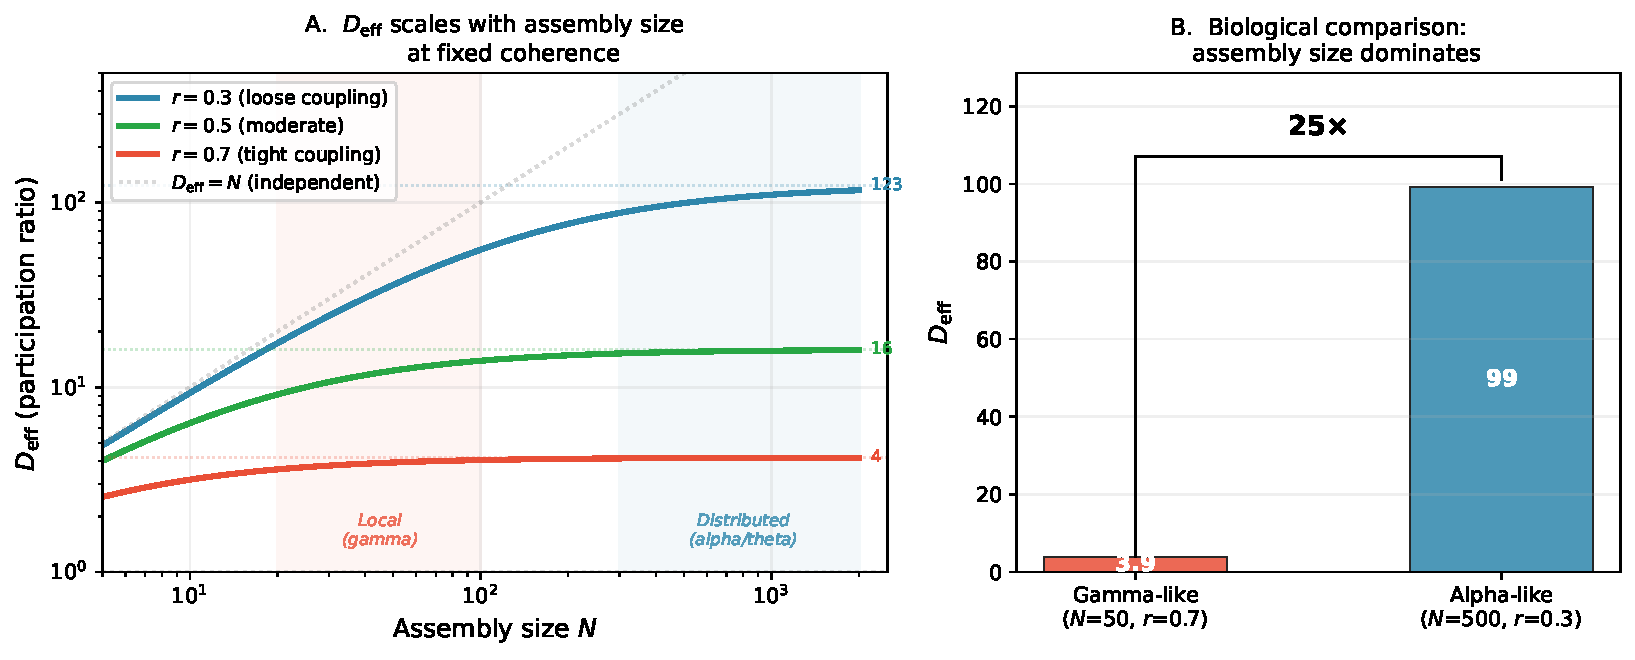
\includegraphics[width=\textwidth]{simulations/figures/fig3.pdf}
\caption{\textbf{Effective dimensionality scales with assembly size at fixed coherence.}
For $N$ oscillators with von Mises distributed phases at coherence $r$, the covariance matrix of $\cos\theta_i$ has compound symmetry (uniform pairwise coherence): $C_{ij} = \frac{1}{2}[(1-r^2)\delta_{ij} + r^2]$, giving participation ratio $\Deff(N, r) = N^2 / [(1 + r^2(N-1))^2 + (N-1)(1-r^2)^2]$. This assumes homogeneous coupling; heterogeneous assemblies would have non-uniform $C_{ij}$ but the qualitative scaling is preserved.
\textbf{(A)}~$\Deff$ vs.\ assembly size $N$ at three coherence levels. Curves saturate at $1/r^4$ (dotted lines): loose coupling ($r = 0.3$) permits $\Deff \approx 123$; tight coupling ($r = 0.7$) saturates at $\Deff \approx 4.2$. Shaded regions indicate biologically relevant regimes for local gamma-band ($N \approx 20$--$100$) and distributed alpha/theta ($N \approx 300$--$2000$) assemblies. Grey diagonal: $\Deff = N$ (independent oscillators).
\textbf{(B)}~Biological comparison: a gamma-like assembly ($N = 50$, $r = 0.7$) achieves $\Deff \approx 3.9$, while an alpha-like assembly ($N = 500$, $r = 0.3$) achieves $\Deff \approx 99$---a $25\times$ fold change driven by the combination of larger spatial extent and looser coupling, supporting the prediction that low-frequency, spatially extensive oscillations sustain higher-dimensional dynamics than local gamma.}
\label{fig:spatial-deff}
\end{figure}

\subsection{Subjective time as experiential dimensionality between commits}
\label{sec:subjective-time}

\textbf{Epistemic status:} This section is exploratory; it translates the framework into falsifiable qualitative predictions about subjective temporal experience across pharmacological conditions.

The coherence time framework establishes that the commit rate
$\Gamma_{\mathrm{commit}} \approx 1/\tau_{\mathrm{coh}}$ is bounded by coordination
dynamics. An immediate consequence concerns the temporal structure of experience.

\subsubsection{The argument}

We build the claim in five steps, intended as a heuristic bridge from the coherence-time framework to phenomenology:

\begin{enumerate}
\item \textbf{Neural dynamics have measurable effective dimensionality.}
This is standard neuroscience: participation ratios, neural manifold analyses, and
related methods quantify $\Deff$ from population recordings~\cite{stringer2019,cunningham2014}.

\item \textbf{Higher $\Deff$ is often associated with richer conscious experience.}
Anaesthesia and dreamless sleep reduce neural complexity. The perturbational complexity
index~\cite{casali2013}, which measures the effective dimensionality of cortical responses
to TMS perturbation, reliably distinguishes conscious from unconscious states in
unresponsive patients. Psychedelics increase neural signal complexity~\cite{timmermann2019,carhart2014}
and produce subjectively enriched experience. This is not yet a general law, but it
motivates the use of $\Deff$ as a candidate experiential variable.

\item \textbf{Commits are bounded below by coherence time}, which scales exponentially
with coordination depth (the central result of this paper, Eq.~\ref{eq:coh-time}).

\item \textbf{If experience depends on high-dimensional dynamics, commit rate should shape temporal grain.}
A commit is a many-to-one map: high-dimensional dynamics collapse to a low-dimensional
readout written to memory, reported verbally, or acted on motorically. On that view, the
temporal structure of experience should depend not only on whether commits occur, but on
the richness of the dynamics between them. Whether experience is best described as the free
exploration between commits or as the high-dimensional convergence \emph{toward} a commit
is an open question; for the predictions below, both framings imply dependence on $\Deff$
and $\Gamma_{\mathrm{commit}}$.

\item \textbf{This motivates the hypothesis that subjective time dilates when $\Deff$ increases relative to commit rate.}
More high-dimensional dynamics are then sampled per commit interval; each interval is
subjectively richer; fewer intervals elapse per second of clock time.
\end{enumerate}

This motivates a simple phenomenological ansatz for subjective temporal scaling:
\begin{equation}\label{eq:subjective-time}
\tau_{\mathrm{subjective}} \propto \frac{\Deff}{\Gamma_{\mathrm{commit}}}
\end{equation}
where $\Gamma_{\mathrm{commit}}$ is bounded by Eq.~\ref{eq:coh-time}. When $\Deff$
increases (more modes active) and $\Gamma_{\mathrm{commit}}$ decreases (harder to
synchronize), the ratio increases---predicting time dilation.

\subsubsection{Pharmacological dissociations}

The framework predicts qualitatively different temporal phenomenology across pharmacological
classes, from the same two-parameter structure ($\Deff$, $\Gamma_{\mathrm{commit}}$; Figure~\ref{fig:pharmacological-space}):

\paragraph{Psychedelics} (5-HT$_{2\mathrm{A}}$ agonists: psilocybin, DMT, LSD).
These increase $\Deff$ by relaxing precision weighting of top-down
priors~\cite{carhart2019rebus}, loosening top-down constraints on dynamics normally
suppressed by hierarchical filtering. They may simultaneously decrease $K/\sigma$ (increased cortical excitability,
disrupted thalamocortical gating). The result is a double effect: higher $\Deff$
\emph{and} lower $\Gamma_{\mathrm{commit}}$, predicting \textbf{time dilation with
experiential richness}. DMT produces large increases in neural signal
complexity under psychedelic perturbation~\cite{timmermann2019,schartner2017} and is associated with
marked subjective time dilation that, at higher doses, can dissolve into reported
timelessness---consistent with a continuum in which increasing $\Deff$ first dilates
temporal experience and eventually overwhelms the commit architecture entirely,
producing a state in which discrete temporal registration ceases to structure
experience. The qualitative ordering---DMT $>$ psilocybin $>$
LSD in both $\Deff$ increase and reported temporal distortion---is consistent with
the prediction, though retrospective magnitude estimates are difficult to validate. \emph{Methodological note:}
retrospective time dilation reports are confounded by altered memory encoding under
psychedelics; increased memory density could inflate retrospective duration estimates
independently of online experience. This framework predicts \emph{online} dilation
($\Deff$ is elevated during the experience), so the critical test requires concurrent
temporal bisection or duration reproduction tasks during drug action, not solely
retrospective report.

\paragraph{Deliriants} (anticholinergics: scopolamine, diphenhydramine).
These increase neural noise ($\sigma$ increases) without structured $\Deff$ increase---
cholinergic disruption degrades organized oscillatory dynamics rather than expanding them.
The prediction is increased commit failure (more noise-dominated measurements) without
increased experiential richness between commits: \textbf{time confusion without time
dilation}. This matches the phenomenology of anticholinergic delirium, where temporal
experience becomes disordered and impoverished rather than expanded.
This is arguably the framework's most discriminating pharmacological prediction: any
generic ``more noise = more subjective time'' account predicts that deliriants and
psychedelics should produce similar temporal distortion (both increase neural entropy).
The $(\Deff, \Gamma_{\mathrm{commit}})$ framework predicts they are qualitatively
different---one expands structured dimensionality, the other injects unstructured noise---
and the phenomenology confirms the distinction.

\paragraph{Anaesthetics} (propofol, sevoflurane).
These likely decrease $\Deff$ by driving the cortex into lower-complexity, less integrative
states~\cite{casali2013}. The prediction is
\textbf{time compression toward unconsciousness}: fewer experiential dimensions per
commit interval, eventually too few for consciousness to be sustained.

\paragraph{Stimulants} (amphetamine, caffeine).
These may increase $\Gamma_{\mathrm{commit}}$ by enhancing oscillatory coupling strength
($K$ increases) without substantially altering $\Deff$. The prediction is
\textbf{mild time expansion with increased temporal resolution}---more commits per
second, each resolving a similar-dimensional state---consistent with the subjective
``speeding up'' reported under moderate stimulant use.

\medskip
The key empirical test distinguishing this framework from generic ``more entropy = altered
time'' accounts: \textbf{subjective time dilation should correlate specifically with the
participation ratio of neural dynamics ($\Deff$), not with broadband entropy.}
Lempel-Ziv complexity and spectral entropy conflate noise and structure---they increase
both when organized modes are added and when random noise is injected. The participation
ratio specifically measures how many independent modes are active, which is what $\Deff$
tracks. A subject whose $\Deff$ doubles should experience greater time dilation than a
subject whose spectral entropy increases by the same amount through noise injection
alone. This prediction is testable with existing pharmacological protocols and
neural recording methods.

\begin{figure}[H]
\centering
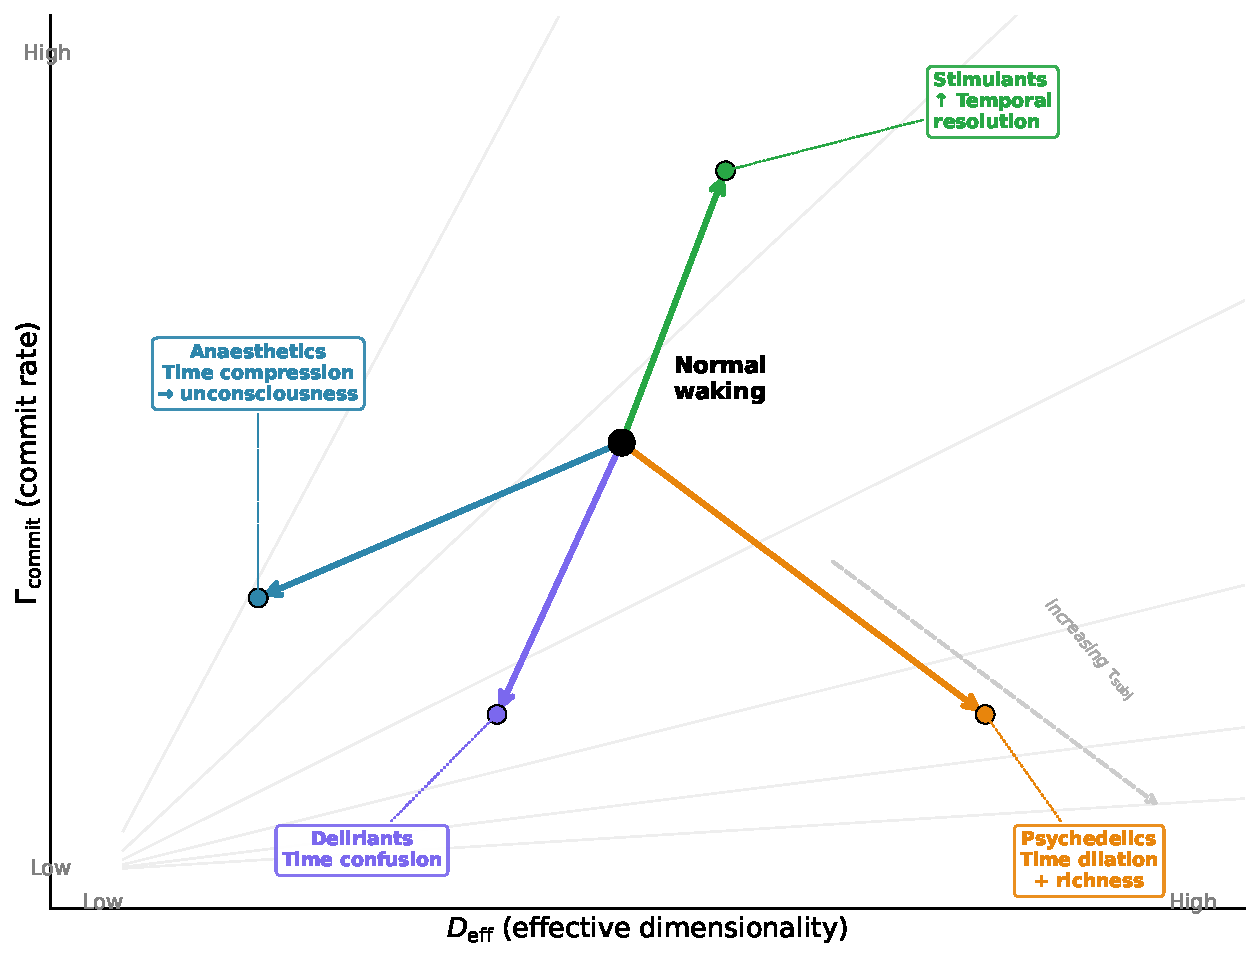
\includegraphics[width=0.85\textwidth]{simulations/figures/fig4.pdf}
\caption{\textbf{Pharmacological prediction space.}
Four drug classes mapped onto the two-parameter space ($\Deff$, $\Gamma_{\mathrm{commit}}$) from a common ``normal waking'' baseline (black dot). Arrows indicate predicted direction of pharmacological perturbation. Grey dashed curves are iso-$\tau_{\mathrm{subj}}$ contours ($\tau_{\mathrm{subj}} \propto \Deff / \Gamma_{\mathrm{commit}}$): movement toward lower-right increases subjective time per clock second; movement toward upper-left compresses it. \textbf{Psychedelics} (orange) increase $\Deff$ and decrease $\Gamma_{\mathrm{commit}}$, predicting time dilation with experiential richness. \textbf{Deliriants} (purple) decrease $\Gamma_{\mathrm{commit}}$ without structured $\Deff$ increase, predicting temporal confusion. \textbf{Anaesthetics} (blue) decrease $\Deff$, predicting time compression toward unconsciousness. \textbf{Stimulants} (green) increase $\Gamma_{\mathrm{commit}}$, predicting increased temporal resolution. The \emph{qualitative quadrant structure} is generated by Eq.~\ref{eq:subjective-time} once a direction of change in $\Deff$ and $\Gamma_{\mathrm{commit}}$ is specified; the quantitative magnitudes of each perturbation arrow remain empirical and drug-specific.}
\label{fig:pharmacological-space}
\end{figure}

\subsubsection{Tachypsychia revisited}

The dual-loop hypothesis of \S3.2 can be reinterpreted within this framework.
During acute stress, arousal increases coherence $r$ in the perceptual loop, which by
the speed-flexibility trade-off (Proposition~\ref{prop:tradeoff}) simultaneously
increases commit \emph{quality} (more information per commit) and may alter commit
\emph{rate} depending on the net effect on $K/\sigma$. The subjective impression of
slowed time during threat reflects increased $\Deff$ of the dynamics being sampled---
heightened arousal activates additional sensory and evaluative modules---while objective
temporal resolution (motor loop) remains unchanged because the motor pathway operates at
low $M$ with different coupling parameters.

\subsection{Implications for artificial and engineered systems}

The coherence time framework identifies a design constraint for any distributed computing system that lacks a global clock. Clocked architectures (CPUs, GPUs) impose synchronization externally, sidestepping the coordination penalty but potentially constraining the kinds of autonomous, semi-independent module dynamics we model here. Unclocked architectures (biological neural networks, neuromorphic hardware) pay the exponential coordination cost but gain access to genuinely high-dimensional dynamics~\cite{todd2025intelligence}. Eq.~\ref{eq:coh-time} provides quantitative guidance for neuromorphic design: such systems must either accept modest $M$, engineer high baseline $r$, or develop hierarchical architectures that localize coordination requirements.

The mammalian cerebellum exemplifies this hierarchical solution. Operating with low coordination depth ($M \sim 3$--5), tight coupling ($r \sim 0.8$), and stereotyped primitives, the cerebellum achieves commit times of 10--20 ms~\cite{wolpert1998,ito2008}---fast enough to override slow cortical dynamics when rapid action is required. Cerebellar processing is largely unconscious, consistent with the hypothesis that phenomenal experience is associated with high-dimensional pre-commit dynamics: the architecture that solves the speed problem---collapsing to low $M$---simultaneously removes processing from the domain of conscious experience.

\subsection{Limitations and scope}

\textbf{Parameter count.} The coherence time bound contains five parameters ($M$, $r$, $\varepsilon$, $\alpha$, $\lambda_{\text{attempt}}$). These should be interpreted as descriptors of coordination architecture rather than unconstrained curve-fitting knobs. This is still a strong compression relative to the full $N$-oscillator system, which has $O(N^2)$ couplings, a frequency distribution, and a noise process. The sparse-topology boundary test is relevant here: when the modular-compression assumption fails, predictive performance degrades as well ($R^2 = 0.28$), indicating that the five-parameter summary has a genuine regime of validity rather than unlimited flexibility.

\textbf{Parameter identifiability.} In the Kuramoto validation, $r$ and $\alpha$ are estimated from simulation data; the remaining parameters are set by model construction. For empirical neural data, simultaneous identifiability of all five parameters from behavioural timing alone is unlikely. The framework is most useful when $M$ and $r$ are constrained independently (e.g., from electrode-array estimates of participating assemblies and pairwise coherence), leaving $\alpha$ as the primary free parameter. Specific predictions jointly constrain parameter subsets: the alpha-entrainment experiment (\S4.3) pins down $\lambda_{\mathrm{attempt}}$ (if binding windows shift linearly with tACS frequency, the proportionality constant gives the attempt rate); the $M$-scaling prediction (exponential dependence across tasks of different coordination depth) pins down $\alpha$; and $\varepsilon$ can be estimated independently from cross-correlogram width. With these three parameters constrained, the remaining degrees of freedom ($M$, $r$) are the task-dependent variables the framework is designed to predict \emph{from}.

\textbf{Regime boundaries.} The exponential scaling $\tau_{\text{coh}} \propto p_1^{-\alpha(M-1)}$ validated cleanly for modular topologies ($R^2 = 0.97$) but poorly for sparse random graphs ($R^2 = 0.28$; Figure~\ref{fig:topology}). This is expected: the bound assumes that inter-module coordination is the rate-limiting step, which requires modular or hierarchical coupling. In networks without clear modular structure, other bottlenecks (percolation thresholds, mixing times) may dominate. The framework therefore applies to systems with identifiable coordination architecture, not to arbitrary oscillator populations.

\textbf{Module-size confound.} The validation sweeps $M$ at fixed $N = 100$, so module size decreases as $M$ increases (from $\sim$33 oscillators at $M = 3$ to 10 at $M = 10$). If within-module coherence $r_{\mathrm{intra}}$ declined with module size, this would provide a competing explanation for the $\tau$ increase. We verified that $r_{\mathrm{intra}}$ does \emph{not} systematically decline: mean $r_{\mathrm{intra}}$ ranges from 0.66 to 0.74 across $M = 3$--$10$ with a slight positive trend (smaller modules synchronize more easily given the same $K_{\mathrm{intra}}$), confirming that the observed $\tau$ scaling with $M$ reflects inter-module coordination cost, not intra-module degradation.

\textbf{Dwell time sensitivity.} The commit detection requires sustained alignment for $T_{\mathrm{dwell}} = 30$~ms. We tested robustness by halving (15~ms) and doubling (60~ms) this threshold: median $\tau_{\mathrm{coh}}$ estimates changed by less than 5\% across all $M$ values, confirming that the first-passage time to initial alignment dominates the estimate and the hold requirement is not doing substantive work. The scaling exponent is robust to $T_{\mathrm{dwell}}$ variation.

\textbf{Relation to synchronisation theory.} The Kuramoto model and its extensions~\cite{kuramoto1984, strogatz2000, acebron2005, ott2008} provide a mature theory of synchronisation onset and order-parameter dynamics. Recent work has extended this framework to excitatory-inhibitory architectures, showing that excitation-inhibition balance can move coupled phase-oscillator systems between synchronized, bistable, and desynchronized regimes~\cite{kuroki2025}. In our interpretation, the coherence time bound is most relevant in partially synchronized regimes where alignment is possible but rare. These regimes also sit naturally alongside recent discussions of criticality as a computational operating point in brain function~\cite{hengen2025}. This paper does not compete with that literature. We address a different question: given that oscillators \emph{can} synchronise, how long must a system wait for a coordination event of depth $M$ to occur? The coherence time bound is a waiting-time result on the product manifold, not a bifurcation analysis of the order parameter.

\textbf{Temporal embedding.} The Results section treats binding windows and perceptual cycles as manifestations of the coherence time bound. This framing is consistent with existing data but not uniquely so---alternative accounts based on inhibitory rebound, attentional sampling, or predictive coding could generate similar timescales. The distinguishing prediction is the \emph{scaling} of temporal resolution with coordination depth $M$, not the absolute timescale.

\section{Conclusion}

We have shown that coherence time---the time required for distributed oscillatory assemblies to achieve sufficient phase alignment for irreversible state registration---scales exponentially with coordination depth $M$ in the modular regime for which the framework is intended. The unified bound $\tau_{\text{eff}} \geq \max[\tau_{\text{QSL}}, \tau_{\text{SNR}}, \tau_{\text{coh}}, \tau_{\text{power}}]$ shows that in the biological neural regime, quantum speed limits and Landauer bounds are not rate-limiting; multi-module coordination provides the binding constraint on processing rate, exceeding quantum floors by approximately eleven orders of magnitude.

The central validated finding is the speed-flexibility trade-off: increasing $M$ exponentially slows commits but expands combinatorial flexibility, while increasing coupling $r$ speeds commits but restricts dynamics to low-dimensional manifolds. The framework recovers binding-window timescales from independently constrained parameters and yields concrete tests of entrainment linearity, modularity dependence, and temporal-resolution scaling with coordination depth. More exploratory extensions---phase-delta dynamics, candidate biophysical substrates, and subjective-time predictions based on $\Deff / \Gamma_{\mathrm{commit}}$---remain hypotheses, but hypotheses that are now explicitly linked to measurable quantities. The primary limitation is the requirement for identifiable modular structure: the exponential scaling validated cleanly for modular topologies ($R^2 = 0.97$) but not for unstructured networks, restricting applicability to systems with hierarchical or modular coordination architecture.

\section*{Data accessibility}

This is a theoretical framework paper. Kuramoto simulation code and parameter estimation workflows are available at \url{https://github.com/todd866/coherence-time-biosystems}.

\section*{Competing interests}

The author has pending intellectual property related to this work. The author declares no competing financial interests or personal relationships that could have appeared to influence the work reported in this paper.

\section*{Declaration of generative AI use}

During preparation the author used Claude Code (Claude Opus 4.6, Anthropic) for literature review, mathematical formulation, coding, and editing. GPT-5.3 (OpenAI) provided critical feedback on mathematical rigor and empirical grounding. All content was reviewed and revised by the author, who takes full responsibility for the published article.

\section*{Funding}

No external funding supported this work.

\section*{Acknowledgments}

The author thanks Abir Igamberdiev and anonymous reviewers at BioSystems for constructive feedback.

\begin{thebibliography}{99}

\bibitem{miller2018}
Miller, E.K., Lundqvist, M., Bastos, A.M. (2018). Working memory 2.0. \textit{Neuron}, 100(2), 463--475.

\bibitem{lundqvist2016}
Lundqvist, M., Rose, J., Herman, P., Brincat, S.L., Buschman, T.J., Miller, E.K. (2016). Gamma and beta bursts underlie working memory. \textit{Neuron}, 90(1), 152--164.

\bibitem{pinotsis2023}
Pinotsis, D.A., Fridman, G., Miller, E.K. (2023). Cytoelectric coupling: Electric fields sculpt neural activity and ``tune'' the brain's infrastructure. \textit{Progress in Neurobiology}, 226, 102465.

\bibitem{fries2015}
Fries, P. (2015). Rhythms for cognition: communication through coherence. \textit{Neuron}, 88(1), 220--235.

\bibitem{singer1999}
Singer, W. (1999). Neuronal synchrony: a versatile code for the definition of relations? \textit{Neuron}, 24(1), 49--65.

\bibitem{lisman2013}
Lisman, J.E., Jensen, O. (2013). The theta-gamma neural code. \textit{Neuron}, 77(6), 1002--1016.

\bibitem{womelsdorf2007}
Womelsdorf, T., et al. (2007). Modulation of neuronal interactions through neuronal synchronization. \textit{Science}, 316(5831), 1609--1612.

\bibitem{engel2001}
Engel, A.K., Fries, P., Singer, W. (2001). Dynamic predictions: oscillations and synchrony in top-down processing. \textit{Nat. Rev. Neurosci.}, 2(10), 704--716.

\bibitem{varela2001}
Varela, F., et al. (2001). The brainweb: phase synchronization and large-scale integration. \textit{Nat. Rev. Neurosci.}, 2(4), 229--239.

\bibitem{fries2005}
Fries, P. (2005). A mechanism for cognitive dynamics: neuronal communication through neuronal coherence. \textit{Trends Cogn. Sci.}, 9(10), 474--480.

\bibitem{todd2025intelligence}
Todd, I. (2026). Intelligence as high-dimensional coherence: The observable dimensionality bound and computational tractability. \textit{BioSystems}, 260, 105704.

\bibitem{landauer1961}
Landauer, R. (1961). Irreversibility and heat generation in the computing process. \textit{IBM J. Res. Dev.}, 5(3), 183--191.

\bibitem{bormashenko2024}
Bormashenko, E. (2024). Landauer bound in the context of minimal physical principles: Meaning, experimental verification, controversies and perspectives. \textit{Entropy}, 26(5), 423.

\bibitem{mandelstam1945}
Mandelstam, L., Tamm, I. (1945). The uncertainty relation between energy and time in non-relativistic quantum mechanics. \textit{J. Phys. (USSR)}, 9, 249--254.

\bibitem{margolus1998}
Margolus, N., Levitin, L.B. (1998). The maximum speed of dynamical evolution. \textit{Physica D}, 120(1--2), 188--195.

\bibitem{khrennikov2021}
Khrennikov, A. (2021). Quantum-like model for unconscious--conscious interaction and emotional coloring of perceptions and other conscious experiences. \textit{BioSystems}, 208, 104471.

\bibitem{igamberdiev2025constraints}
Igamberdiev, A.U., Shklovskiy-Kordi, N.E. (2025). Physical limits of natural computation as the biological constraints of morphogenesis, evolution, and consciousness: On the 100th anniversary of Efim Liberman (1925--2011). \textit{BioSystems}, 251, 105451.

\bibitem{igamberdiev2026autopoietic}
Igamberdiev, A.U. (2026). Internal quantum constraints of natural computation in autopoietic systems. \textit{BioSystems}, 261, 105707.

\bibitem{khrennikov2025bridge}
Khrennikov, A., Iriki, A., Basieva, I. (2025). Constructing a bridge between functioning of oscillatory neuronal networks and quantum-like cognition along with quantum-inspired computation and AI. \textit{BioSystems}, 257, 105573.

\bibitem{poor1994}
Poor, H.V. (1994). \textit{An Introduction to Signal Detection and Estimation} (2nd ed.). Springer-Verlag.

\bibitem{kac1947}
Kac, M. (1947). On the notion of recurrence in discrete stochastic processes. \textit{Bull. Amer. Math. Soc.}, 53(10), 1002--1010.

\bibitem{mardia2000}
Mardia, K.V., Jupp, P.E. (2000). \textit{Directional Statistics}. John Wiley \& Sons.

\bibitem{stetson2007}
Stetson, C., Fiesta, M.P., Eagleman, D.M. (2007). Does time really slow down during a frightening event? \textit{PLoS ONE}, 2(12), e1295.

\bibitem{samaha2015}
Samaha, J., Postle, B.R. (2015). The speed of alpha-band oscillations predicts the temporal resolution of visual perception. \textit{Current Biology}, 25(22), 2985--2990.

\bibitem{cecere2015}
Cecere, R., Rees, G., Romei, V. (2015). Individual differences in alpha frequency drive crossmodal illusory perception. \textit{Current Biology}, 25(2), 231--235.

\bibitem{healy2013}
Healy, K., McNally, L., Ruxton, G.D., Cooper, N., Jackson, A.L. (2013). Metabolic rate and body size are linked with perception of temporal information. \textit{Anim. Behav.}, 86(4), 685--696.

\bibitem{tononi2016}
Tononi, G., Boly, M., Massimini, M., Koch, C. (2016). Integrated information theory: from consciousness to its physical substrate. \textit{Nat. Rev. Neurosci.}, 17(7), 450--461.

\bibitem{friston2010}
Friston, K. (2010). The free-energy principle: a unified brain theory? \textit{Nat. Rev. Neurosci.}, 11(2), 127--138.

\bibitem{anastassiou2011}
Anastassiou, C.A., Perin, R., Markram, H., Koch, C. (2011). Ephaptic coupling of cortical neurons. \textit{Nat. Neurosci.}, 14(2), 217--223.

\bibitem{beggs2003}
Beggs, J.M., Plenz, D. (2003). Neuronal avalanches in neocortical circuits. \textit{J. Neurosci.}, 23(35), 11167--11177.

\bibitem{shew2013}
Shew, W.L., Plenz, D. (2013). The functional benefits of criticality in the cortex. \textit{Neuroscientist}, 19(1), 88--100.

\bibitem{han2018}
Han, K.S., Guo, C., Chen, C.H., Witter, L., Osorno, T., Regehr, W.G. (2018). Ephaptic coupling promotes synchronous firing of cerebellar Purkinje cells. \textit{Neuron}, 100(3), 564--578.

\bibitem{kuramoto1984}
Kuramoto, Y. (1984). \textit{Chemical Oscillations, Waves, and Turbulence}. Springer-Verlag, Berlin.

\bibitem{strogatz2000}
Strogatz, S.H. (2000). From Kuramoto to Crawford: exploring the onset of synchronization in populations of coupled oscillators. \textit{Physica D}, 143(1-4), 1--20.

\bibitem{acebron2005}
Acebr\'{o}n, J.A., Bonilla, L.L., P\'{e}rez Vicente, C.J., Ritort, F., and Spigler, R. (2005). The Kuramoto model: A simple paradigm for synchronization phenomena. \textit{Reviews of Modern Physics}, 77(1), 137--185.

\bibitem{ott2008}
Ott, E. and Antonsen, T.M. (2008). Low dimensional behavior of large systems of globally coupled oscillators. \textit{Chaos}, 18(3), 037113.

\bibitem{cunningham2014}
Cunningham, J.P. and Yu, B.M. (2014). Dimensionality reduction for large-scale neural recordings. \textit{Nature Neuroscience}, 17(11), 1500--1509.

\bibitem{stringer2019}
Stringer, C., Pachitariu, M., Steinmetz, N., Reddy, C.B., Carandini, M., and Harris, K.D. (2019). Spontaneous behaviors drive multidimensional, brainwide activity. \textit{Science}, 364(6437), eaav7893.

\bibitem{todd2025biosystems}
Todd, I. (2025). The limits of falsifiability: Dimensionality, measurement thresholds, and the sub-Landauer domain in biological systems. \textit{BioSystems}, 258, 105608.

\bibitem{todd2025demon}
Todd, I. (2025). Timing inaccessibility and the projection bound: Resolving Maxwell's demon for continuous biological substrates. \textit{BioSystems}, 258, 105632.

\bibitem{raichle2001}
Raichle, M.E., MacLeod, A.M., Snyder, A.Z., Powers, W.J., Gusnard, D.A., and Shulman, G.L. (2001). A default mode of brain function. \textit{Proceedings of the National Academy of Sciences}, 98(2), 676--682.

\bibitem{wolpert1998}
Wolpert, D.M., Miall, R.C., and Kawato, M. (1998). Internal models in the cerebellum. \textit{Trends in Cognitive Sciences}, 2(9), 338--347.

\bibitem{vanrullen2016}
VanRullen, R. (2016). Perceptual cycles. \textit{Trends in Cognitive Sciences}, 20(10), 723--735.

\bibitem{helfrich2014}
Helfrich, R.F., Schneider, T.R., Rach, S., Trautmann-Lengsfeld, S.A., Engel, A.K., and Herrmann, C.S. (2014). Entrainment of brain oscillations by transcranial alternating current stimulation. \textit{Current Biology}, 24(3), 333--339.

\bibitem{amari2016}
Amari, S. (2016). \textit{Information Geometry and Its Applications}. Springer, Tokyo.

\bibitem{ashby1956}
Ashby, W.R. (1956). \textit{An Introduction to Cybernetics}. Chapman \& Hall, London.

\bibitem{levinperes2017}
Levin, D.A., Peres, Y. (2017). \textit{Markov Chains and Mixing Times} (2nd ed.). American Mathematical Society.

\bibitem{ito2008}
Ito, M. (2008). Control of mental activities by internal models in the cerebellum. \textit{Nat. Rev. Neurosci.}, 9(4), 304--313.

\bibitem{casali2013}
Casali, A.G., Gosseries, O., Rosanova, M., Boly, M., Sarasso, S., Casali, K.R.,
Casarotto, S., Bruno, M.-A., Laureys, S., Tononi, G., and Massimini, M. (2013).
A theoretically based index of consciousness independent of sensory processing and
behavior. \textit{Science Translational Medicine}, 5(198), 198ra105.

\bibitem{timmermann2019}
Timmermann, C., Roseman, L., Schartner, M., Milliere, R., Williams, L.T.J.,
Erritzoe, D., Muthukumaraswamy, S., Ashton, M., Bendrioua, A., Kaelen, M.,
Brugger, M., Williams, S., Bolstridge, M., Feilding, A., Nutt, D.J., and
Carhart-Harris, R.L. (2019). Neural correlates of the DMT experience assessed with
multivariate EEG. \textit{Scientific Reports}, 9, 16324.

\bibitem{carhart2014}
Carhart-Harris, R.L., Leech, R., Hellyer, P.J., Shanahan, M., Feilding, A.,
Tagliazucchi, E., Chialvo, D.R., and Nutt, D. (2014). The entropic brain: a theory
of conscious states informed by neuroimaging research with psychedelic drugs.
\textit{Frontiers in Human Neuroscience}, 8, 20.

\bibitem{carhart2019rebus}
Carhart-Harris, R.L. and Friston, K.J. (2019). REBUS and the anarchic brain: toward a
unified model of the brain action of psychedelics. \textit{Pharmacological Reviews},
71(3), 316--344.

\bibitem{schartner2017}
Schartner, M.M., Carhart-Harris, R.L., Barrett, A.B., Seth, A.K., and
Muthukumaraswamy, S.D. (2017). Increased spontaneous MEG signal diversity for
psychoactive doses of ketamine, LSD and psilocybin. \textit{Scientific Reports},
7, 46421.

\bibitem{buzsaki2004}
Buzs\'{a}ki, G. and Draguhn, A. (2004). Neuronal oscillations in cortical networks.
\textit{Science}, 304(5679), 1926--1929.

\bibitem{kuroki2025}
Kuroki, S. and Mizuseki, K. (2025). Excitation--inhibition balance controls
synchronization in a simple model of coupled phase oscillators.
\textit{Neural Computation}, 37(7), 1353--1372.

\bibitem{hengen2025}
Hengen, K.B. and Shew, W.L. (2025). Is criticality a unified setpoint of brain
function? \textit{Neuron}, 113(16), 2545--2570.

\bibitem{wutz2024}
Wutz, A. (2024). Alpha oscillations create the illusion of time.
\textit{Journal of Cognitive Neuroscience}, 36(4), 712--720.

\end{thebibliography}

\end{document}
